%==============================================================================
%  Device-Free Human Motion Detection Using Wi-Fi Channel State Information
%  and an ESP32-S3
%
%  Engineering / Projet de Fin d'Etudes (PFE) report.
%
%  ---------------------------------------------------------------------------
%  HOW TO COMPILE ON OVERLEAF
%  ---------------------------------------------------------------------------
%  1. Create a new blank project and upload this file.
%  2. Create a folder named  figures/  and upload into it every PNG from
%     report_output/figures/  in the repository. The report uses:
%         01_confusion_matrix.png             13_class_distribution.png
%         02_confusion_matrix_normalized.png  14_learning_curve.png
%         03_train_vs_test_by_fold.png        15_validation_curve.png
%         04_test_accuracy_by_fold.png        16_calibration_curve.png
%         05_boxplot_fold_accuracies.png      17_prediction_probability_histogram.png
%         09_roc_curve.png                    20_fold_performance_summary.png
%         10_pr_curve.png                     21_waterfall_empty_vs_moving.png
%         11_feature_importance_top20.png     22_motion_energy_transition.png
%         12_cumulative_feature_importance.png 23_class_separation_quiet_vs_loud.png
%                                             24_noise_floor_per_session.png
%                                             25_noise_floor_vs_accuracy.png
%                                             26_feature_importance_by_family.png
%                                             27_empty_room_character.png
%     (Regenerate them with:  python full_model_report.py --model csi_model.joblib
%      --sessions <the ten>   then   python make_report_figures.py)
%  3. Set the compiler to pdfLaTeX (Menu > Compiler) and compile TWICE so the
%     table of contents, list of figures and cross-references settle.
%
%  Every package used here ships with a standard TeX Live / Overleaf install.
%  No shell-escape and no external downloads are required.
%
%  ---------------------------------------------------------------------------
%  IF A FIGURE IS MISSING
%  ---------------------------------------------------------------------------
%  Set \figuresmissingtrue below and the document will compile with labelled
%  placeholder boxes instead of images, so you can work on the text before the
%  figures are uploaded.
%==============================================================================

\documentclass[11pt,a4paper,oneside]{report}

%------------------------------------------------------------------ packages --
\usepackage[utf8]{inputenc}
\usepackage[T1]{fontenc}
\usepackage[english]{babel}
% Change "Chapter" to "Part" throughout the document
\usepackage[margin=2.5cm,headheight=14pt]{geometry}

\usepackage{amsmath}
\usepackage{amssymb}
\usepackage{graphicx}
\usepackage{booktabs}
\usepackage{longtable}
\usepackage{array}
\usepackage{tabularx}
\usepackage{multirow}
\usepackage{caption}
\usepackage{float}
\usepackage{enumitem}
\usepackage{xcolor}
\usepackage{listings}
\usepackage{fancyhdr}
\usepackage{titlesec}
\usepackage{etoolbox}



\usepackage{tikz}
\usetikzlibrary{arrows.meta, positioning, shapes.geometric, fit, calc, backgrounds}

\usepackage[colorlinks=true,
            linkcolor=blue!45!black,
            urlcolor=blue!45!black,
            citecolor=blue!45!black]{hyperref}
\hypersetup{
  pdftitle={Device-Free Human Motion Detection Using Wi-Fi Channel State Information and an ESP32-S3},
  pdfsubject={Wi-Fi sensing, embedded machine learning},
  pdfkeywords={Wi-Fi sensing, CSI, ESP32, device-free sensing, Random Forest, OFDM}
}

%--------------------------------------------------------- figure fallback ----
\newif\iffiguresmissing
\figuresmissingfalse   % <-- set to \figuresmissingtrue to compile without images

\graphicspath{{figures/}{./figures/}{report_output/figures/}{../report_output/figures/}{./}}

% Include a figure, or a labelled placeholder if figures are unavailable.
% \detokenize in the placeholder branch is required, not cosmetic: the file
% names contain underscores, which are harmless as an \includegraphics argument
% but would be read as subscripts if typeset as ordinary text.
\newcommand{\projfig}[2]{%
  \iffiguresmissing
    \fbox{\parbox[c][3.2cm][c]{0.9\linewidth}{\centering\ttfamily\small
      figure not uploaded: \detokenize{#2}}}%
  \else
    \includegraphics[width=#1\linewidth]{#2}%
  \fi
}

%------------------------------------------------------------------- styling --
\definecolor{codebg}{RGB}{246,246,244}
\definecolor{accent}{RGB}{15,98,208}
\definecolor{good}{RGB}{21,127,61}
\definecolor{bad}{RGB}{194,53,47}
\definecolor{warn}{RGB}{162,104,11}
\definecolor{neutralgrey}{RGB}{90,92,98}
\definecolor{rulegrey}{RGB}{120,120,120}

\lstdefinestyle{codestyle}{
  backgroundcolor=\color{codebg},
  basicstyle=\ttfamily\footnotesize,
  breaklines=true,
  frame=single,
  framerule=0.3pt,
  rulecolor=\color{rulegrey},
  xleftmargin=6pt,
  aboveskip=10pt,
  belowskip=6pt,
  keywordstyle=\color{accent}\bfseries,
  commentstyle=\color{good}\itshape,
  stringstyle=\color{warn},
  showstringspaces=false,
  tabsize=2,
  captionpos=b,
}
\lstset{style=codestyle}

\pagestyle{fancy}
\fancyhf{}
\fancyhead[L]{\small\itshape\leftmark}
\fancyhead[R]{\small\thepage}
\renewcommand{\headrulewidth}{0.3pt}
\renewcommand{\chaptermark}[1]{\markboth{\chaptername\ \thechapter.\ #1}{}}

\titleformat{\chapter}[display]
  {\normalfont\huge\bfseries}{\chaptertitlename\ \thechapter}{16pt}{\Huge}
\titlespacing*{\chapter}{0pt}{-18pt}{28pt}

%------------------------------------------------------- evidence-class tags --
% Every substantive claim in this report carries one of these tags, so a reader
% can always separate what the system does from what was measured, what the
% measurement means, and what is only proposed.
% NOTE: this macro must NOT be called \tag. amsmath already defines \tag for
% manual equation numbering, so \newcommand{\tag} aborts with "Command \tag
% already defined" and every later use then fails with "\tag not allowed here".
\newcommand{\evidencetag}[2]{{\small\sffamily\bfseries\textcolor{#1}{[#2]}}}
\newcommand{\Impl}{\evidencetag{good}{Implemented}}
\newcommand{\Meas}{\evidencetag{accent}{Measured}}
\newcommand{\Repo}{\evidencetag{neutralgrey}{Reported by the repository}}
\newcommand{\Theo}{\evidencetag{warn}{Theoretical}}
\newcommand{\Fut}{\evidencetag{bad}{Proposed Future Work}}

\newcommand{\code}[1]{\texttt{\small #1}}
\newcommand{\keyfinding}[1]{%
  \begin{center}\fbox{\begin{minipage}{0.94\linewidth}\vspace{3pt}#1\vspace{3pt}\end{minipage}}\end{center}}
\newcommand{\blank}{\rule{5cm}{0.4pt}}

\captionsetup{font=small, labelfont=bf}

%==============================================================================
\begin{document}
%==============================================================================

%------------------------------------------------------------- title page --%------------------------------------------------------------- title page ----
\begin{titlepage}

% ============================================================
%                    PAGE STYLE
% ============================================================
\thispagestyle{empty}

% ============================================================
%                    UNIVERSITY / COMPANY LOGOS
% ============================================================
\vspace*{0.3cm}

\begin{minipage}[c]{0.44\textwidth}
    \raggedright
    \includegraphics[
        height=2.8cm,
        keepaspectratio
    ]{logo.png}
\end{minipage}
\hfill
\begin{minipage}[c]{0.44\textwidth}
    \raggedleft
    \includegraphics[
        height=2.8cm,
        keepaspectratio
    ]{eidia.jpg}
\end{minipage}

\vspace{0.9cm}

% ============================================================
%                    TOP ACCENT LINE
% ============================================================
\noindent
\color{accent}\rule{\textwidth}{1.5pt}

\vspace{0.8cm}

% ============================================================
%                    REPORT TYPE
% ============================================================
\begin{center}

{\large
    \color{neutralgrey}
    \textsc{\bfseries End-of-Year Project}
}

\vspace{0.15cm}

{\normalsize
    \color{neutralgrey}
    \textsc{Engineering Internship Report}
}

\vspace{1.0cm}
\end{center}
% ============================================================
%                    MAIN TITLE
% ============================================================
\begin{center}
{\fontsize{27}{32}\selectfont
    \bfseries
    \color{accent!90!black}
    Device-Free Human Motion Detection
}

\vspace{0.45cm}

{\fontsize{17}{22}\selectfont
    \bfseries
    \color{neutralgrey}
    A Wi-Fi CSI-Based Intrusion Detection System
}

\vspace{0.25cm}

{\fontsize{15}{20}\selectfont
    \color{neutralgrey}
    Using the ESP32-S3
}

\vspace{0.8cm}
\end{center}
% ============================================================
%                    ACCENT DIVIDER
% ============================================================
\begin{center}
\color{accent}
\rule{0.22\textwidth}{2pt}

\vspace{0.7cm}
\end{center}
% ============================================================
%                 UNIVERSITY / COMPANY LOGOS
% ============================================================
\begin{center}
\begin{minipage}[c]{0.44\textwidth}
    \centering
    \includegraphics[
        height=4.0cm,
        keepaspectratio
    ]{logo_company.jpg}
\end{minipage}
\end{center}

% ============================================================
%                     PROJECT INFORMATION
% ============================================================

\vspace{1cm}

\noindent
\begin{minipage}[t]{0.48\textwidth}
    \raggedright
    {\small\scshape\bfseries\color{accent} Prepared by}\\[0.3cm]
    \textbf{Student:} Ilyass Arro \\[0.15cm]
    \textbf{University:} Euro-Mediterranean University of Fes (UEMF)
\end{minipage}%
\hfill
\begin{minipage}[t]{0.48\textwidth}
    \raggedright
    {\small\scshape\bfseries\color{accent} Supervised by}\\[0.3cm]
    \textbf{Host Company:} MULTINOVA, Meknès \\[0.15cm]
    \textbf{Supervisor:} Dr. Mohammed EL ALAMI
\end{minipage}

\vfill

% ============================================================
%                    BOTTOM INFORMATION
% ============================================================

\noindent
\color{accent}\rule{\textwidth}{0.8pt}

\vspace{0.25cm}

\begin{center}

{\small
    \color{neutralgrey}
    \textsc{Academic Year 2025--2026}
    \qquad
    \textbullet
    \qquad
    \today
}

\end{center}

\end{titlepage}


\pagenumbering{roman}

% ---- Acknowledgements ----
% ---- Acknowledgements (styled like the sample: title framed by two flourishes)
% Put the two decorative images in  images/ :  UP.png  and  DOWN.jpg .
% (\IfFileExists is used so the file still compiles even before you add them.)
\clearpage
\thispagestyle{plain}
\addcontentsline{toc}{chapter}{Acknowledgements}
\markboth{Acknowledgements}{Acknowledgements}

\begin{center}
  {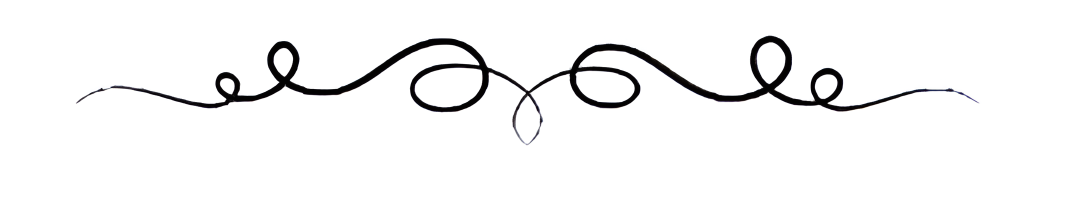
\includegraphics[width=0.42\textwidth]{UP.png}\\[0.35cm]}{}%
  {\Huge\itshape Acknowledgements}\\[0.30cm]
\end{center}
\vspace{0.8cm}

% Block-style paragraphs (no first-line indent, clear vertical spacing between
% them) for a clean, well-organised look. The group keeps this local to the
% acknowledgements page; the rest of the report is unaffected.
\begingroup
\setlength{\parindent}{0pt}
\setlength{\parskip}{0.9em}

I would like to express my sincere gratitude to everyone who contributed, directly
or indirectly, to the successful completion of this internship and this report.

I would first like to express my deepest gratitude to my supervisor, Dr. Mohammed El Alami, for his attentive guidance, constant availability, and valuable advice throughout this project. I am especially grateful for his expertise, patience, insightful feedback, and for everything he taught me during this experience.


I would also like to express my sincere gratitude to all my professors at the
\textbf{School of Digital Engineering and Artificial Intelligence (EIDIA)} of
\textbf{Euromed University of Fez (UEMF)}, whose dedication, academic excellence, and continuous support played a significant role in the development of my knowledge and skills and contributed greatly to the successful completion of this project.

I warmly thank \textbf{Professor Ahmed EL HILALI ALAOUI}, Director of EIDIA, for
his inspiring vision, his leadership, and his constant commitment to excellence in
education. My sincere thanks likewise go to \textbf{Professor Badr ELKARI}, Head
of the Robotics and Cobotics track,for his guidance, his availability, and his valuable support throughout my studies.

Finally, I express my heartfelt gratitude to my family and loved ones for their
moral support and their constant encouragement throughout this formative
experience.
 
\par\endgroup
\begin{center}
  {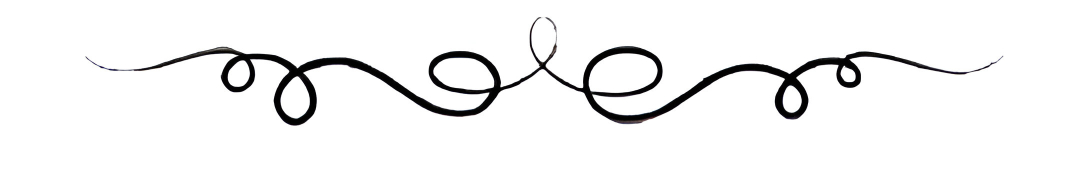
\includegraphics[width=0.42\textwidth]{DOWN.jpg}}{}%
\end{center}
%--------------------------------------------------------- source of record ---
\chapter*{Source of Record}
\addcontentsline{toc}{chapter}{Source of Record}
\markboth{Source of Record}{}

This report documents the project hosted at
\url{https://github.com/IALR/csi-motion-detection}. Every quantitative claim was
taken from the repository's source code, datasets and trained model, or
re-derived by running the project's own scripts. Statements are labelled
throughout so that the reader can always distinguish what the system currently
does from what was measured, what the measurements mean, and what remains
future work:

\begin{center}
\begin{tabularx}{0.94\linewidth}{@{}lX@{}}
\toprule
\Impl & The behaviour exists in the committed source code. \\
\Meas & A number obtained by executing the project's scripts on the committed data. \\
\Repo & A value or event documented in the repository's development history. \\
\Theo & A statement of physics or method, not a measurement of this system. \\
\Fut  & Not built; proposed. \\
\bottomrule
\end{tabularx}
\end{center}

\noindent
No experimental result in this report was fabricated. Where the repository does
not provide a value, this is stated explicitly and left as a placeholder rather
than estimated.

\medskip
\noindent

%------------------------------------------------------------------ abstract --
\chapter*{Abstract}
\addcontentsline{toc}{chapter}{Abstract}
\markboth{Abstract}{}

Detecting whether a person is moving inside an indoor space, without a camera,
a wearable, or a dedicated sensor mounted on the person, is a useful capability
for building automation, security and assisted living. Each conventional
sensing modality carries a significant drawback: cameras raise privacy
concerns, passive-infrared detectors miss a stationary or slowly moving person,
and wearables require cooperation from the subject. This project investigates
device-free motion detection using Wi-Fi Channel State Information (CSI), a
fine-grained measurement of how the wireless channel distorts a signal across
its OFDM subcarriers, which every Wi-Fi receiver already computes internally in
order to equalise incoming data. The physical premise is that a moving person
perturbs the multipath propagation between a transmitter and a receiver, and
that this perturbation is visible in the temporal variation of CSI amplitude.

A single ESP32-S3 microcontroller extracts CSI from its link to an ordinary
Wi-Fi access point, computes per-subcarrier amplitude on-device, and streams it
over a serial link. A Python pipeline expresses each short time window of
amplitudes relative to a freshly measured empty-room baseline, extracts 266
features combining per-subcarrier statistics with room-agnostic aggregate
summaries, and classifies each window as empty or moving using a Random Forest.
The model was validated with leave-one-session-out cross-validation across ten
recording sessions in two rooms, achieving \textbf{94.25\,\%} per-window
accuracy (weighted, out-of-fold) with balanced errors: \textbf{107} false
alarms and \textbf{83} missed detections across 3\,302 windows.

The dominant limitation, established by the project's own measurements rather
than asserted, is environmental dependence: the empty-room radio-frequency
noise floor varies by approximately a factor of nine between sessions, and
held-out accuracy ranges from 84.67\,\% to 98.69\,\% accordingly. A further
measurement presented here shows that the noisy sessions are not uniformly
noisy but \emph{intermittent}: in the worst session the empty room has a median
frame-to-frame energy of 1.20 against a mean of 5.06, with 42\,\% of empty
frames bursting to levels indistinguishable from human movement. The system
performs motion detection only --- not presence, localisation or tracking ---
and has been trained and tested on a single person's movement. The most
valuable next step is collecting movement data from additional people, to test
whether the model detects \emph{a} person rather than \emph{this} person.

\medskip
\noindent
\textbf{Keywords:} Wi-Fi sensing; Channel State Information (CSI); ESP32;
device-free sensing; human motion detection; OFDM; Random Forest; signal
processing; embedded systems; leave-one-session-out validation.

%--------------------------------------------------------------- front matter -
\tableofcontents
\listoffigures
\listoftables

\chapter*{Abbreviations}
\addcontentsline{toc}{chapter}{Abbreviations}
\markboth{Abbreviations}{}

\begin{center}
\begin{tabularx}{\linewidth}{@{}lX@{}}
\toprule
\textbf{Abbreviation} & \textbf{Meaning} \\
\midrule
AP        & Access Point \\
BSSID     & Basic Service Set Identifier (an access point's MAC address) \\
CSI       & Channel State Information \\
DC        & Direct Current (the zero-frequency subcarrier) \\
ESP-IDF   & Espressif IoT Development Framework \\
FN / FP   & False Negative / False Positive \\
HT-LTF    & High Throughput Long Training Field \\
I/Q       & In-phase / Quadrature components of a complex sample \\
L-LTF     & Legacy Long Training Field \\
LOS / NLOS& Line-of-Sight / Non-Line-of-Sight \\
LOSO      & Leave-One-Session-Out (cross-validation) \\
MAC       & Medium Access Control (address / layer) \\
MCC       & Matthews Correlation Coefficient \\
ML        & Machine Learning \\
OFDM      & Orthogonal Frequency-Division Multiplexing \\
RF        & Radio Frequency, or Random Forest (disambiguated in the text) \\
RSSI      & Received Signal Strength Indicator \\
SNR       & Signal-to-Noise Ratio \\
UART      & Universal Asynchronous Receiver/Transmitter \\
Wi-Fi     & IEEE 802.11 wireless local-area networking \\
\bottomrule
\end{tabularx}
\end{center}

%==============================================================================
\chapter{Introduction}
%==============================================================================
\section{Presentation of the company}

MULTINOVA Énergie is an engineering-oriented company based in Meknès, Morocco, operating mainly in the fields of renewable energy, energy efficiency, electrical engineering and automation. Under the direction of Mr. Mohammed El Alami, the company develops and implements technical solutions adapted to the energy and industrial requirements of its clients. Its activities include the study and installation of photovoltaic systems, solar-powered irrigation solutions, electrical installations and automated systems, combining engineering studies with practical implementation. Through this multidisciplinary approach, MULTINOVA Énergie operates at the intersection of renewable energy, electrical systems, automation and intelligent technologies, with the objective of improving the efficiency, reliability and sustainability of technical installations. This professional environment provides an appropriate setting for engineering students to apply theoretical knowledge to real-world projects while developing practical skills in electrical engineering, electronics, automation, embedded systems and energy management.

\begin{figure}[H]
\centering
\projfig{1.0}{MUlti.jpg}
\caption{ MULTINOVA Énergie}
\label{fig:waterfall}
\end{figure}

\begin{table}[H]
\centering
\caption[Fact sheet of MULTINOVA \'Energie]{Fact sheet of MULTINOVA \'Energie.}
\label{tab:multinova-factsheet}
\renewcommand{\arraystretch}{1.25}
\begin{tabularx}{\linewidth}{|>{\raggedright\arraybackslash}p{4.3cm}|X|}
\hline
Field & Value \\
\hline
Company name & MULTINOVA Énergie \\
\hline
Legal status & SARL à associé unique \\
\hline
Director / Manager & M. Mohammed El Alami \\
\hline
Business area & Renewable energy, energy efficiency, electrical installations, engineering studies and automation \\
\hline
Main activities & Photovoltaic systems, solar-powered irrigation, electrical systems, automation and technical studies \\
\hline
Location & Meknès, Morocco \\
\hline
Address & Avenue Mohammed VI, Résidence Oum Rabie, N°112, 3ème étage, Appartement 9, Meknès \\
\hline
Main technical fields & Renewable energy, electrical engineering, automation, electronics and energy systems \\
\hline
Main focus & Design, study and implementation of technical and energy solutions \\
\hline
Target applications & Energy supply, photovoltaic installations, irrigation systems and intelligent technical solutions \\
\hline
\end{tabularx}
\end{table}
\section{Background}

Indoor sensing is important for applications such as building automation, security, energy management, and assisted living. Conventional solutions have limitations: cameras raise privacy concerns, PIR sensors mainly detect movement, dedicated ultrasonic or microwave sensors add hardware costs, and wearables require user cooperation.

Wireless sensing offers a different approach by using existing Wi-Fi signals to sense changes in the environment. Since the human body reflects, absorbs, and scatters radio waves, human movement changes the wireless channel between radios. By measuring these changes, Wi-Fi infrastructure can be used for device-free indoor motion detection without cameras or wearable devices. 

\section{Problem Statement}

The problem addressed by this project is narrow and precisely defined:

\keyfinding{\centering Given a single low-cost Wi-Fi receiver in an indoor room,
decide in real time whether the room is \textbf{empty} or whether a person is
\textbf{moving} in it, using only the wireless channel, with no camera and no
device carried by the person.}

\noindent
This is challenging for reasons the project encountered directly. The wireless
channel changes for many reasons that have nothing to do with a person  a
neighbouring network's traffic, an air-conditioning unit switching on, thermal
drift in the hardware, or the access point renegotiating its channel width. The
signal that betrays a moving person is small relative to these nuisance
variations, and its magnitude depends on where the person is relative to the
transmitter--receiver line. A method that works in one room, on one day, with
one hardware placement, may not transfer to another. Much of the engineering
effort in this project, documented in later chapters, was spent not on the
classifier but on separating genuine motion from environmental change.

\section{Motivation}

Wi-Fi CSI is an attractive basis for device-free sensing for four concrete
reasons.

\begin{enumerate}[leftmargin=1.6em, itemsep=3pt]
  \item \textbf{The infrastructure already exists.} Wi-Fi access points are
        present in almost every indoor environment, and CSI is a by-product
        that every OFDM receiver computes internally to equalise the channel.
        No new transmitter is required. \Theo
  \item \textbf{The hardware is inexpensive.} This project uses a single
        ESP32-S3 module costing a few euros, in contrast to the specialised
        network cards historically needed to expose CSI on commodity
        computers. \Impl
  \item \textbf{The sensing is device-free and non-contact.} Nothing is mounted
        on the person; the room itself is the sensor. \Impl
  \item \textbf{Relative to a camera, CSI avoids direct visual capture.} This
        must be stated carefully. CSI is \emph{not} automatically
        privacy-preserving: it does not record an image, which removes one
        obvious class of harm, but wireless channel measurements can reveal
        surprisingly detailed information about people. The correct claim is
        that it avoids the specific privacy problems of a camera, not that it
        is private. This distinction is developed in Chapter~\ref{ch:privacy}.
\end{enumerate}

\section{Objectives}

\subsection*{Primary objectives}

The project aimed to acquire Wi-Fi CSI using an ESP32, extract motion-related features, train a classifier to distinguish between empty and moving states, and perform real-time detection. All core components were implemented and validated.. \Impl

\subsection*{Secondary objectives}

The project also aimed to improve robustness to environmental changes, provide real-time visualisation, support multi-node sensing, and evaluate cross-room generalisation. These objectives were implemented to varying degrees, with cross-room testing limited to two rooms. Generalisation to different rooms and people remains an open challenge.

\section{Contributions}

\textbf{Hardware and firmware.} A self-contained ESP32-S3 firmware that
extracts CSI, generates its own CSI-triggering traffic by pinging the gateway,
filters CSI to the associated access point, pins the link to a 20\,MHz channel
width so the subcarrier count stays fixed at 128, and streams amplitudes over
serial without stalling the radio. \Impl

\textbf{Software architecture.} A single shared module (\code{csi\_common.py})
that is the sole source of truth for parsing, feature extraction and
calibration, imported identically by the offline training path and both live
paths so that the two cannot silently diverge. \Impl

\textbf{Signal processing.} A calibration scheme expressing every window
relative to a recent empty-room baseline  amplitude means as deltas, spreads
as ratios  recalibrated per empty block offline and through a
blended-and-floored rolling calibrator online, together with a set of
order-invariant band-summary features intended to transfer across rooms. \Impl

\textbf{Machine learning.} A Random Forest classifier selected by comparison
against five other model families under identical validation, with its
stability, feature importances and failure modes characterised in detail. 

\textbf{Experimental.} A ten-session dataset across two rooms, validated with
leave-one-session-out cross-validation, and  unusually  a documented,
honest analysis of when and why the model fails, tying held-out accuracy to a
measured empty-room noise floor rather than reporting only the best number.
\Meas

%==============================================================================
\chapter{State of the Art and Theoretical Background}
\label{ch:sota}
%==============================================================================

\section{Traditional Human Sensing}

Traditional sensing methods involve different trade-offs. Cameras provide rich information but raise privacy concerns and depend on lighting and line of sight. PIR sensors are inexpensive and low-power but mainly detect movement. Ultrasonic sensors can detect presence and distance but are affected by environmental conditions. Radar provides robust motion detection but requires dedicated hardware, while wearables offer accurate per-person sensing but require user cooperation. \Theo

\section{Wi-Fi as a Sensing Modality}

Human movement affects Wi-Fi signals by reflecting, absorbing, and changing the multipath propagation between devices. Since Wi-Fi hardware already measures the wireless channel, these measurements can be reused for sensing without additional hardware. Two common measurements are RSSI, which provides overall received signal strength, and CSI, which provides detailed channel information across individual subcarriers. \Theo

\section{RSSI-Based Sensing}

RSSI is a simple measure of received signal power that changes when a person moves. However, because it reduces the complex multipath channel to a single value, it is noisy and provides limited information.

In this project, RSSI is used only as two auxiliary features alongside CSI. Feature-importance analysis showed that the calibrated RSSI spread ratio was the most important individual feature, while raw RSSI alone was insufficient. This highlights the importance of calibration when using RSSI for sensing. \Meas

\section{CSI-Based Human Sensing}

CSI exposes the channel's complex response at each OFDM subcarrier, giving tens
to hundreds of values per frame instead of one. Because different subcarriers
experience multipath differently, CSI captures fine-grained, frequency-selective
channel structure that RSSI discards.

The research literature built on CSI spans a spectrum of tasks of increasing
difficulty:

\begin{center}
\begin{tabularx}{0.92\linewidth}{@{}lX@{}}
\toprule
\textbf{Task} & \textbf{Question answered} \\
\midrule
Motion detection      & Is anything moving? \quad \textit{(this project)} \\
Presence / occupancy  & Is anyone there, moving or not? \\
Activity recognition  & Walking, sitting, falling? \\
Gesture recognition   & Which gesture was performed? \\
Localisation          & Where is the person? \\
Tracking              & How does that position evolve? \\
Vital signs           & Breathing and heart rate from chest motion \\
\bottomrule
\end{tabularx}
\end{center}

\noindent
This project sits at the easiest, most robust end of that spectrum  binary
motion detection  and does not attempt activity recognition, localisation or
tracking. This is a deliberate scoping choice, and the terminology distinction
is maintained throughout the report.

\section{Existing CSI Systems}

Representative systems in the literature illustrate the design space along
several axes: the CSI source (early work used the Intel 5300 and Atheros
network cards on PCs; more recent work, including this project, uses the ESP32,
which exposes CSI cheaply on a microcontroller); the number of antennas and
links (multi-antenna receivers expose spatial diversity and usable phase,
single-antenna devices such as the ESP32 do not); the features (raw amplitude,
denoised amplitude, calibrated phase, Doppler and velocity spectra); and the
model (fixed thresholds, classical machine learning such as Random Forests and
support vector machines, or deep networks).

The consistent finding across this literature and the one most relevant
here is that CSI sensing performance is strongly dependent on environment
and hardware, and that generalisation across rooms, people and devices is the
central open challenge, not the raw classification accuracy in a fixed setting.
This project's own results reproduce exactly that pattern.

\begin{quote}\small
\textbf{Note on citations.} The systems and results referenced in this chapter
are described generically because the project itself did not perform a formal
literature review with reproducible citations. The bibliography lists only
sources actually used during implementation. Before submission, add proper
citations for the representative systems in this area; the References chapter
names specific families of work to look up.
\end{quote}

\section{Research Gap and Positioning}

This project does not claim novelty of concept: ESP32 CSI motion detection with
classical machine learning is an established idea. Its contribution is instead
one of engineering rigour and honesty on a low-cost platform  a fully
reproducible single-module pipeline; a calibration scheme designed specifically
against the environment-dependence that the literature flags as the core
problem; order-invariant features aimed at cross-room transfer; and, most
distinctively, a measurement-driven account of when the system fails and why,
in which held-out accuracy is tied to a quantified empty-room noise floor
rather than summarised by a single favourable number.

The project explicitly does \emph{not} claim to be first at anything, nor to
have solved cross-room, cross-person or cross-device generalisation.

%==============================================================================

%==============================================================================

\section{Wi-Fi Fundamentals}

Wi-Fi (IEEE 802.11) transmits data over unlicensed radio bands, principally
2.4\,GHz and 5\,GHz, divided into channels. A channel has a nominal width 
20\,MHz, 40\,MHz or wider --- and the width directly determines how many OFDM
subcarriers occupy the channel, and therefore how many CSI values a receiver
reports.

This relationship is not a background detail in this project; it is
load-bearing:

\keyfinding{A \textbf{20\,MHz} link causes the ESP32 to report
\textbf{128} amplitude values per frame; a \textbf{40\,MHz} link causes it to
report \textbf{192}. The classifier is built for a fixed input dimensionality,
so an access point that silently renegotiates its channel width breaks the
feature vector outright. \Impl\ \Repo}

\noindent
The firmware therefore pins the station's link to 20\,MHz
(Chapter~\ref{ch:fw}), fixing the count at 128. This failure occurred three
separate times during development before being fixed at the source. \Repo

\section{OFDM}

Wi-Fi uses Orthogonal Frequency-Division Multiplexing: rather than sending data
on one wideband carrier, it divides the channel into many narrow, mutually
orthogonal subcarriers, each carrying a fraction of the data in parallel. Two
properties matter here.

First, splitting a wide channel into narrow subcarriers turns a
frequency-selective wideband channel into many approximately flat narrowband
channels, each of which can be equalised with a single complex coefficient 
and that per-subcarrier coefficient \emph{is} CSI.

Second, not all subcarriers carry data. Guard bands at the channel edges and a
DC null at the centre are left empty to limit interference and hardware
impairments. These structurally empty subcarriers report essentially zero
amplitude and, as shown in Chapter~\ref{ch:dsp}, cause a subtle but serious
numerical problem in ratio-based features if not handled. \Theo

\begin{figure}[H]
\centering
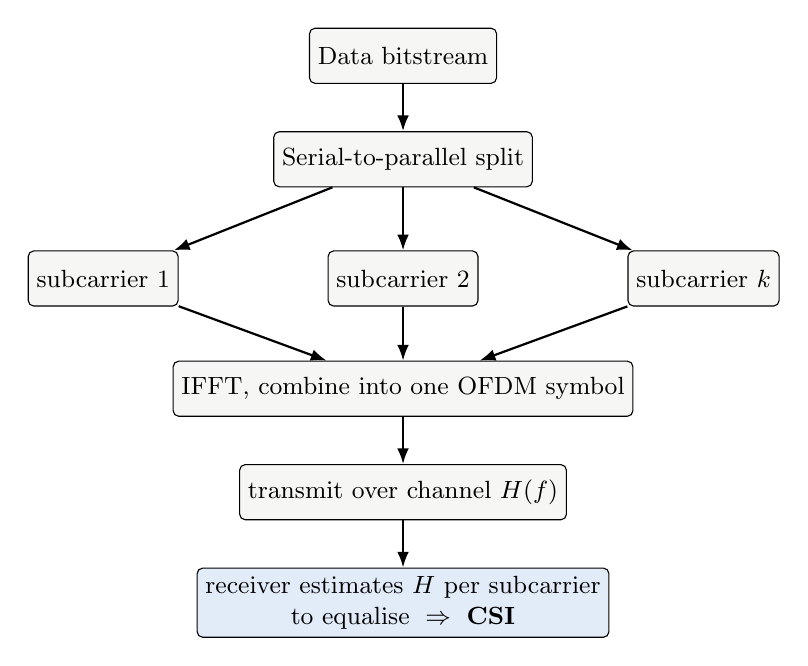
\begin{tikzpicture}[font=\small, node distance=6mm,
  b/.style={draw, rounded corners=2pt, align=center, minimum height=7mm,
            inner sep=3pt, fill=codebg},
  a/.style={-{Latex[length=2mm]}, thick}]
\node[b] (bits) {Data bitstream};
\node[b, below=of bits] (sp) {Serial-to-parallel split};
\node[b, below left=8mm and 12mm of sp] (s1) {subcarrier 1};
\node[b, below=8mm of sp] (s2) {subcarrier 2};
\node[b, below right=8mm and 12mm of sp] (sk) {subcarrier $k$};
\node[b, below=22mm of sp] (ifft) {IFFT, combine into one OFDM symbol};
\node[b, below=of ifft] (chan) {transmit over channel $H(f)$};
\node[b, below=of chan, fill=accent!12] (csi) {receiver estimates $H$ per subcarrier\\to equalise $\;\Rightarrow\;$ \textbf{CSI}};
\draw[a] (bits) -- (sp);
\draw[a] (sp) -- (s1); \draw[a] (sp) -- (s2); \draw[a] (sp) -- (sk);
\draw[a] (s1) -- (ifft); \draw[a] (s2) -- (ifft); \draw[a] (sk) -- (ifft);
\draw[a] (ifft) -- (chan);
\draw[a] (chan) -- (csi);
\end{tikzpicture}
\caption[OFDM subcarrier structure and the origin of CSI]{OFDM distributes data
across parallel narrowband subcarriers. The per-subcarrier channel estimate the
receiver computes in order to equalise them is the Channel State Information.}
\label{fig:ofdm}
\end{figure}

\section{The Wireless Channel}

A signal radiated from a transmit antenna reaches the receiver not by one path
but by many: a direct line-of-sight component may arrive alongside reflections
off walls, floor, ceiling and furniture, diffraction around edges, and
scattering off rough or small objects. Each path has its own length, and
therefore its own delay and phase, and its own attenuation. At the receiver
these components sum coherently, and because they can add constructively or
destructively depending on their relative phases, the resulting channel is
\emph{frequency-selective} (different subcarriers are affected differently)
and, in the presence of anything moving, \emph{time-varying}. \Theo

\begin{figure}[H]
\centering
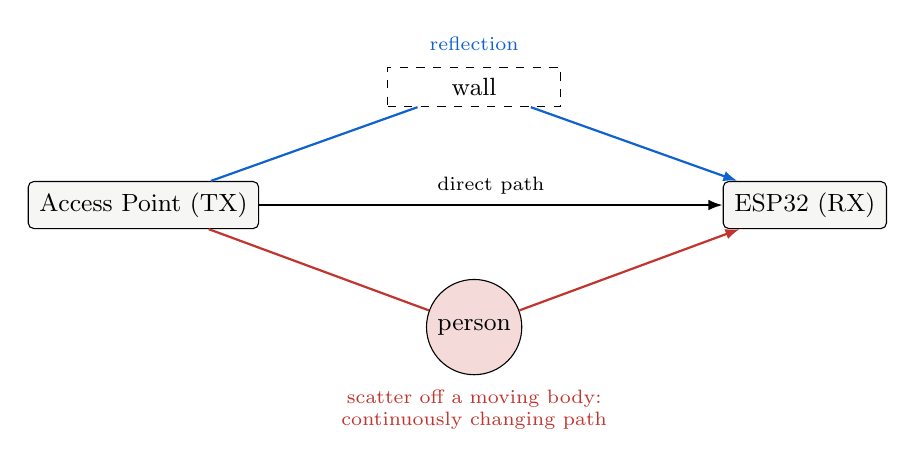
\begin{tikzpicture}[font=\small,
  dev/.style={draw, rounded corners=2pt, fill=codebg, inner sep=4pt},
  p/.style={-{Latex[length=1.8mm]}, thick}]
\node[dev] (ap) at (0,0) {Access Point (TX)};
\node[dev] (rx) at (8.4,0) {ESP32 (RX)};
\node[draw, circle, fill=bad!18, inner sep=3pt] (per) at (4.2,-1.55) {person};
\node[draw, dashed, minimum width=2.2cm, minimum height=5mm] (wall) at (4.2,1.5) {wall};
\draw[p] (ap) -- node[above, font=\scriptsize] {direct path} (rx);
\draw[p, accent] (ap) -- (wall) -- (rx);
\node[font=\scriptsize, accent] at (4.2,2.05) {reflection};
\draw[p, bad] (ap) -- (per) -- (rx);
\node[font=\scriptsize, bad, align=center] at (4.2,-2.6) {scatter off a moving body:\\continuously changing path};
\end{tikzpicture}
\caption[Multipath propagation and human perturbation]{Multipath propagation. A
moving person adds and continuously changes reflected and scattered components,
perturbing the summed channel observed at the receiver.}
\label{fig:multipath}
\end{figure}

\section{Channel State Information}

Consider a single OFDM subcarrier. If $X$ is the transmitted symbol, $Y$ the
received symbol, $H$ the complex channel response on that subcarrier and $N$
additive noise, then to first order
\begin{equation}
  Y = H X + N .
  \label{eq:channel}
\end{equation}
To recover $X$ the receiver must estimate $H$; that estimate, taken across all
subcarriers, is the Channel State Information. Written as a function of
subcarrier index, $H(f)$ is a vector of complex numbers describing how the
channel attenuates and phase-shifts each subcarrier. CSI is therefore a far
richer description of the channel than RSSI, which is approximately a single
scalar summarising $\sum_f |H(f)|^2$.

\section{Complex CSI, Amplitude and Phase}

Each subcarrier's channel response is complex,
\begin{equation}
  H_k = A_k + j B_k ,
\end{equation}
with amplitude and phase
\begin{equation}
  |H_k| = \sqrt{A_k^2 + B_k^2}, \qquad
  \varphi_k = \operatorname{atan2}(B_k, A_k).
  \label{eq:amp}
\end{equation}

The ESP32 delivers, per subcarrier, an imaginary and a real signed 8-bit
integer. \textbf{This project uses amplitude only.} The firmware computes
$|H_k| = \operatorname{round}\!\left(\sqrt{\mathrm{imag}^2 +
\mathrm{real}^2}\right)$ and discards the phase before anything leaves the
board. \Impl

This is a deliberate and consequential choice. Raw CSI phase from a single,
unsynchronised commodity receiver is corrupted by carrier-frequency offset,
sampling-time offset and random phase-lock-loop offsets, and is not usable
without a sanitisation step that a single-antenna ESP32 cannot support.
Discarding phase sidesteps that corruption but also forecloses any technique
that needs phase --- most importantly, angle- and range-based localisation
(Chapter~\ref{ch:limits}). \Theo

\subsection*{On the count of 128}

The firmware computes \code{n = len / 2} amplitude values from a raw CSI buffer
of \code{len} bytes, one value per interleaved (imaginary, real) pair, and
reports \code{n} in the \code{num\_subcarriers} field. Measured across all ten
sessions, this field is \textbf{128} in every frame. \Meas\ The firmware's own
buffer constant documents that a 40\,MHz link produces 384 bytes, i.e.\ 192
values. \Impl

Since the CSI configuration enables both the legacy and the high-throughput
long training fields with merging (Chapter~\ref{ch:fw}), a count of
$128 = 2 \times 64$ at 20\,MHz is consistent with the buffer containing both
estimates. This interpretation is stated as such and is not required by any
result in this report: the pipeline treats the 128 values as an ordered vector
of per-frame amplitudes, approximately twenty of which are structurally dead.
\Theo

\section{Human Motion and CSI}

When the room is static the multipath channel is static, so CSI amplitude is
approximately constant frame to frame, varying only with noise. When a person
moves they continuously change the geometry of the reflected and scattered
paths, so the summed channel  and therefore CSI amplitude on the affected
subcarriers  fluctuates over time. The detectable quantity is thus the
\emph{temporal variation} of CSI amplitude, not its absolute value:
\begin{center}
\fbox{%
  \colorbox{codebg}{%
    \begin{minipage}{0.92\linewidth}
      \vspace{4pt}
      \centering
      \small\sffamily
      \textbf{\color{accent}Core Wi-Fi Sensing Principle}\\[0.4em]
      $\text{Static Environment} \implies \text{Stationary Multipath} \implies \mathbf{\text{Constant CSI}}$\\[0.3em]
      $\text{Human Motion} \implies \text{Dynamic Phase \& Reflection} \implies \mathbf{\color{accent}\text{Amplitude Fluctuation}}$
      \vspace{4pt}
    \end{minipage}%
  }%
}
\end{center}

This is directly observable in the project's own recordings.
Figure~\ref{fig:waterfall} shows raw amplitude over time for the same session,
with the room empty and with a person moving. In the empty panel each
subcarrier holds a steady value, producing smooth vertical banding; in the
moving panel that banding is broken up by continuous temporal disruption.

\begin{figure}[H]
\centering
\projfig{1.0}{21_waterfall_empty_vs_moving.png}
\caption[Raw CSI amplitude, empty versus moving]{Raw CSI amplitude over time
for \code{part\_1\_data}, 150 frames of each class on a shared colour scale.
Horizontal axis: active subcarrier index. Vertical axis: time. An empty room
produces stable per-subcarrier values; a moving person disrupts them
continuously. \Meas}
\label{fig:waterfall}
\end{figure}

\section{Why Motion Can Be Detected Without Seeing the Person}

Device-free sensing works because the person does not need to transmit, be
seen, or be instrumented; they only need to exist in the propagation
environment. Their body is an obstacle and reflector that changes how the
transmitter's signal reaches the receiver. The receiver never ``sees'' the
person; it observes that the channel it shares with the access point is
behaving differently from how an empty room behaves. Detection is thus an
inference about the channel, from which the presence of motion is deduced 
never a direct observation of the person.

\section{Project Management}
\label{sec:project-management}

The work was organised in an iterative way, in short cycles built around a record–evaluate–correct loop: each cycle delivered a system that ran end to end and was validated before the next began first serial capture and a labelled dataset, then feature extraction and calibration, the Random Forest with its leave-one-session-out validation, live inference and the browser dashboard, the second node and its OR fusion, and finally the standalone firmware port. The ordering deliberately front-loaded the risk, so that the question capable of ending the project whether amplitude-only CSI is separable at all — was answered on real recordings in the third week, before any effort was committed to the dashboard, the second node or the embedded deployment. Because every recording session was evaluated as soon as it was captured, defects in the protocol surfaced inside the cycle that produced them rather than at the end: several sessions were re-recorded on that basis and one early exploratory dataset was discarded outright, which is why data collection and modelling overlap in the schedule instead of running in sequence.

\subsection{Schedule: Gantt Chart}
\label{subsec:gantt}

The project schedule was laid out as a Gantt chart, breaking the internship
down into weekly iterations and making the dependencies between successive
increments explicit.

\begin{figure}[H]
\centering
\projfig{0.95}{28_project_timeline.png}
\caption[Project schedule  Gantt chart]{Project schedule. Each bar
corresponds to one weekly iteration, ordered so that every increment left the
tool in a runnable state before the next began. \Repo}
\label{fig:gantt}
\end{figure}


%==============================================================================
\chapter{System Requirements, Architecture and Hardware Implementation}
\label{ch:arch}
%==============================================================================

\section{Functional Requirements}

The system must acquire CSI continuously from a live Wi-Fi link, stream it to a
processing host (or process it on-device), transform each short time window into
a calibrated feature vector, classify that window as empty or moving, smooth the
prediction against single-window noise, and present the result in real time.
Each of these is implemented; the mapping to source files is given in
Chapter~\ref{ch:live} and Appendix~\ref{app:files}. \Impl

\section{Non-Functional Requirements}

The system is designed for real-time, low-cost, and privacy-preserving operation, with approximately 10 Hz processing and sub-second response time. It emphasizes reproducibility, robustness to environmental changes through calibration, and scalability to multiple sensing nodes. The classifier must also be computationally efficient enough to run on either a PC or directly on the ESP32.

\section{Overall Architecture}

The deployed data path is a linear pipeline from the access point to a
prediction, with an optional second node combined at the very end.

\begin{figure}[H]
\centering
% Make sure these libraries are in your preamble:
% \usetikzlibrary{arrows.meta, positioning, calc}
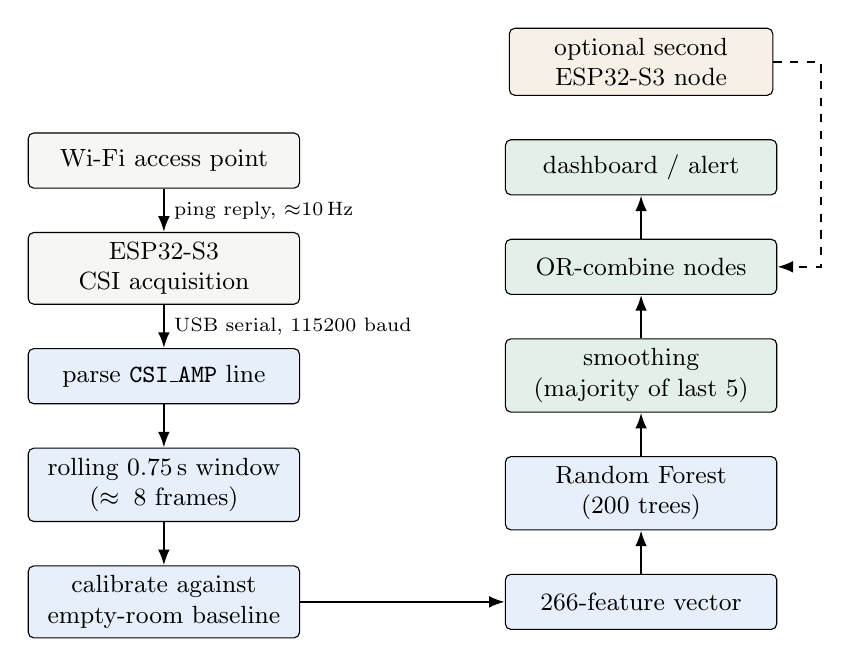
\begin{tikzpicture}[
  font=\small,
  node distance=5.5mm,
  b/.style={draw, rounded corners=2pt, align=center, minimum height=7mm,
            inner sep=3.5pt, fill=codebg, text width=3.2cm},
  p/.style={draw, rounded corners=2pt, align=center, minimum height=7mm,
            inner sep=3.5pt, fill=accent!10, text width=3.2cm},
  o/.style={draw, rounded corners=2pt, align=center, minimum height=7mm,
            inner sep=3.5pt, fill=good!12, text width=3.2cm},
  a/.style={-{Latex[length=2mm]}, thick}
]

% ---- Column 1: top -> bottom ----
\node[b] (ap) {Wi-Fi access point};
\node[b, below=of ap] (esp) {ESP32-S3\\CSI acquisition};
\node[p, below=of esp] (parse) {parse \code{CSI\_AMP} line};
\node[p, below=of parse] (win) {rolling 0.75\,s window\\($\approx 8$ frames)};
\node[p, below=of win] (cal) {calibrate against\\empty-room baseline};

% ---- Column 2: bottom -> top, starts level with cal ----
\node[p, right=26mm of cal] (feat) {266-feature vector};
\node[p, above=of feat] (rf) {Random Forest\\(200 trees)};
\node[o, above=of rf] (sm) {smoothing\\(majority of last 5)};
\node[o, above=of sm] (fuse) {OR-combine nodes};
\node[o, above=of fuse] (out) {dashboard / alert};

% ---- main flow ----
\draw[a] (ap) -- node[right, font=\scriptsize] {ping reply, $\approx$10\,Hz} (esp);
\draw[a] (esp) -- node[right, font=\scriptsize] {USB serial, 115200 baud} (parse);
\draw[a] (parse) -- (win);
\draw[a] (win) -- (cal);
\draw[a] (cal) -- (feat);   % column wrap
\draw[a] (feat) -- (rf);
\draw[a] (rf) -- (sm);
\draw[a] (sm) -- (fuse);
\draw[a] (fuse) -- (out);

% ---- optional second node, above, merging down into OR-combine ----
\node[b, above=of out, text width=3.1cm, fill=warn!10] (esp2)
  {optional second\\ESP32-S3 node};
\draw[a, dashed] (esp2.east) -- ++(6mm,0) |- (fuse.east);

\end{tikzpicture}
\caption[Overall system architecture]{Overall system architecture. The optional
second node runs an identical, fully independent pipeline; only the final
confirmed states are combined. \Impl}
\label{fig:arch}
\end{figure}

\section{Data Flow}

A CSI frame originates when a packet arrives at the ESP32. Because CSI only
exists when packets flow, the firmware manufactures a steady packet stream by
pinging the gateway every 100\,ms, yielding roughly ten CSI frames per second.
Each frame passes through the Wi-Fi driver's CSI callback, which copies it into
a queue; a separate task formats it as an ASCII \code{CSI\_AMP} line and writes
it to the UART. On the host, the line is parsed into an RSSI value and 128
amplitudes, appended to a rolling buffer and  once the buffer holds a full
0.75\,s window  converted to a calibrated 266-feature vector, classified and
smoothed. With two nodes, each maintains its own buffer, baseline and
prediction, and the server combines the two confirmed states. \Impl

\section{Hardware/Software Separation}

In the primary configuration the ESP32 performs acquisition only: it captures
CSI, computes amplitude, filters to the associated access point and streams.
All windowing, calibration, feature extraction, classification and smoothing
occur on the host. This division keeps the firmware simple and lets the
compute-heavy and frequently-changed parts live in Python, where they are easy
to modify and validate.

The project later demonstrated (Chapter~\ref{ch:live}) that the same model can
be exported to C and executed standalone on the ESP32, moving inference
on-device while training remains on the PC. The standalone path is single-node
and does not change the architecture described here. \Impl

%==============================================================================

\label{ch:hw}
%==============================================================================

\section{The ESP32-S3}

The sensing node is an ESP32-S3, a low-cost microcontroller with an integrated
2.4\,GHz Wi-Fi radio, a dual-core Xtensa LX7 processor and importantly for
this project a driver that exposes per-packet CSI to application code. The
specific board used was found to carry 16\,MB of flash and 8\,MB of PSRAM,
considerably more than the 2\,MB the default build configuration assumed; this
headroom is what later made on-device inference feasible. \Repo

The ESP32-S3 is suitable here because it combines a CSI-capable Wi-Fi stack,
enough compute and memory for optional on-device inference, and a UART for
streaming, at a cost of a few euros  the economic premise of the whole
approach. Only specifications confirmed from the repository and vendor
documentation are asserted; where a precise figure was not established, it is
not invented.

\section{The Wi-Fi Access Point}

The access point is an ordinary Wi-Fi router (or, during some bring-up, a phone
hotspot). Its role is not to provide Internet connectivity but to be the other
end of the wireless link whose channel is being measured, and to generate the
traffic via ping replies that causes CSI to be produced.

The access point's configuration matters: if it negotiates a 40\,MHz channel
width, the reported count doubles from 128 to 192 and breaks the model. This
occurred three times during development and was ultimately fixed on the station
side by pinning the link to 20\,MHz in firmware. \Repo

\section{Hardware Setup}

A typical deployment places the ESP32 and the access point at fixed positions
in a room, with the person moving in the space between and around them. Exact
distances, room dimensions and line-of-sight geometry are \textbf{not recorded
numerically in the repository} and are therefore left as placeholders to be
completed from the student's own notes:

\begin{table}[H]
\centering
\caption{Physical deployment parameters.}
\label{tab:deployment_parameters}
\begin{tabularx}{0.8\linewidth}{@{}Xl@{}}
\toprule
\textbf{Setup parameter} & \textbf{Value} \\
\midrule
Room 1 dimensions              & $3\,\mathrm{m} \times 5\,\mathrm{m}$ ($15\,\mathrm{m^2}$) \\
Room 2 dimensions              & $3\,\mathrm{m} \times 3\,\mathrm{m}$ ($9\,\mathrm{m^2}$) \\
ESP32 to access point distance & $3\,\mathrm{m}$ \\
ESP32 / access point height    & $1\,\mathrm{m}$ / $1.2\,\mathrm{m}$ \\
Line-of-sight (LOS / NLOS)     & LOS \\
Person's movement area         & Central area of the room \\
\bottomrule
\end{tabularx}
\end{table}

\noindent

\section{Hardware Components}

\begin{table}[H]
\centering
\caption{Hardware components.}
\label{tab:hw}
\renewcommand{\arraystretch}{1.25}
\begin{tabularx}{\linewidth}{|l|X|X|}
\hline
\textbf{Component} & \textbf{Purpose} & \textbf{Important characteristics} \\
\hline
ESP32-S3 module &
CSI acquisition, amplitude computation, serial streaming, optional on-device
inference &
2.4\,GHz Wi-Fi with CSI callback; dual-core Xtensa LX7; 16\,MB flash and 8\,MB
PSRAM on the board used; single antenna \\
\hline
Wi-Fi access point &
Far end of the measured link; source of CSI-triggering traffic &
Should permit a fixed 20\,MHz channel width; a phone hotspot works but cannot
be pinned from its own side \\
\hline
Host PC &
Windowing, calibration, features, classification, dashboard &
Python 3 with the dependencies in \code{requirements.txt}; one exclusive serial
port per node \\
\hline
USB cable &
Power and UART link &
115200 baud; the same cable powers a standalone deployment from a charger \\
\hline
Second ESP32-S3 (optional) &
Second sensing node covering a different geometry &
Combined by OR logic at the host; must not be co-located with the first \\
\hline
\end{tabularx}
\end{table}

\section{Single-Node Architecture}

The baseline system is a single ESP32 streaming to a single host process. One
node observes one transmitter--receiver geometry and therefore has a
characteristic blind region: a person moving along a path that barely perturbs
that particular link is harder to detect. This is a property of single-link CSI
physics, not a software defect. \Impl

\section{Multi-Node Architecture}

To mitigate the single-link blind region, the project added a second ESP32
node. The two nodes are deliberately \emph{not} co-located placing them
together would have them observe nearly identical multipath and defeat the
purpose. Each node runs an entirely independent pipeline (its own serial link,
baseline, window and model inference), and the host combines only the two
confirmed states using OR logic: the room is reported MOVING if either node
reports MOVING, and EMPTY only if every participating node reports EMPTY
(Chapter~\ref{ch:live}).

This is an implemented, live-validated capability. It is a \emph{coverage}
improvement, not a localisation system: the two nodes are not synchronised and
their measurements are never jointly triangulated. \Impl

%==============================================================================

\label{ch:fw}
%==============================================================================

All statements in this chapter are taken from
\code{firmware/main/csi\_node.c} and the accompanying firmware sources.

\section{Firmware Architecture}

The firmware runs a small number of cooperating tasks. On boot it optionally
runs a self-test (Chapter~\ref{ch:live}), initialises non-volatile storage,
Wi-Fi and the event loop, connects as a station, pins the link to 20\,MHz,
creates a CSI queue and a printer task, starts a periodic ping to generate
traffic, arms the optional on-device detector, and finally enables CSI.

The design principle is that the time-critical Wi-Fi callback does as little as
possible, handing work to a separate task through a queue.

\begin{figure}[H]
\centering
% Preamble additions needed for this version:
% \usetikzlibrary{arrows.meta, positioning, calc, fit, backgrounds}
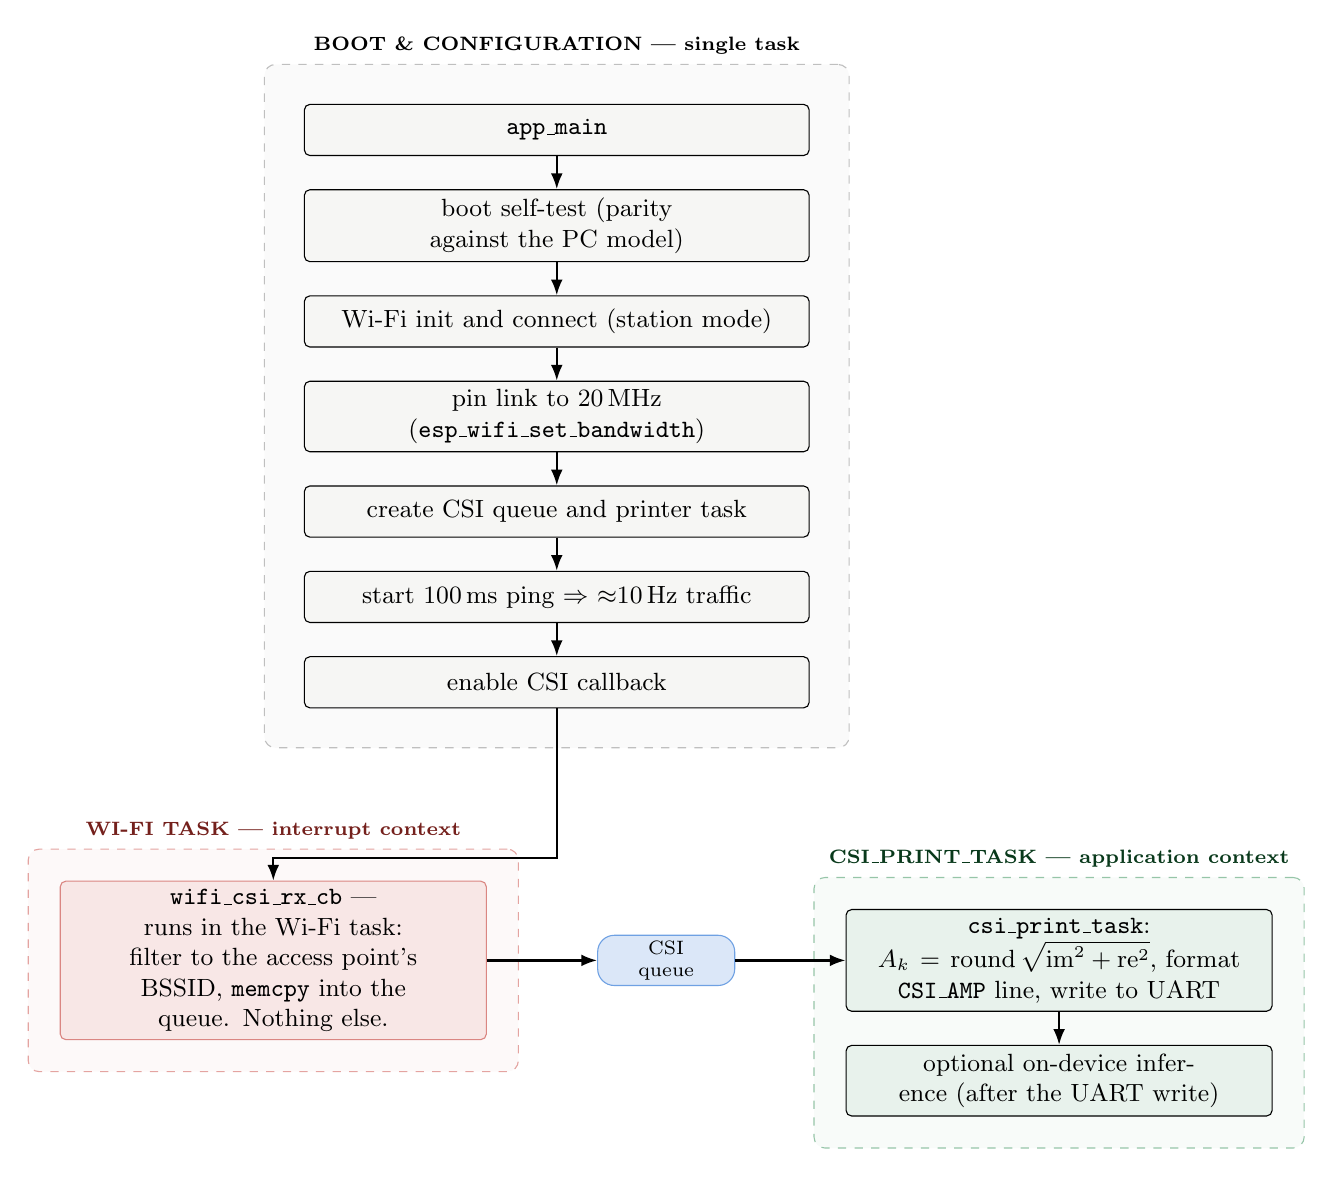
\begin{tikzpicture}[
  font=\small,
  node distance=4.2mm and 9mm,
  b/.style={draw, rounded corners=2pt, align=center, minimum height=6.5mm,
            inner sep=3pt, fill=codebg, text width=6.2cm},
  h/.style={draw, rounded corners=2pt, align=center, minimum height=6.5mm,
            inner sep=3pt, fill=bad!12, draw=bad!60, text width=5.2cm},
  t/.style={draw, rounded corners=2pt, align=center, minimum height=6.5mm,
            inner sep=3pt, fill=good!10, text width=5.2cm},
  q/.style={draw, rounded corners=6pt, align=center, minimum height=6mm,
            inner sep=2pt, fill=accent!15, draw=accent!60, font=\scriptsize,
            text width=1.6cm},
  a/.style={-{Latex[length=2mm]}, thick},
  lbl/.style={font=\scriptsize\bfseries}
]

% ---------- Phase 1: sequential boot / init ----------
\node[b] (n1) {\code{app\_main}};
\node[b, below=of n1] (n2) {boot self-test (parity against the PC model)};
\node[b, below=of n2] (n3) {Wi-Fi init and connect (station mode)};
\node[b, below=of n3] (n4) {pin link to 20\,MHz (\code{esp\_wifi\_set\_bandwidth})};
\node[b, below=of n4] (n5) {create CSI queue and printer task};
\node[b, below=of n5] (n6) {start 100\,ms ping $\Rightarrow$ $\approx$10\,Hz traffic};
\node[b, below=of n6] (n7) {enable CSI callback};

\foreach \i/\j in {n1/n2,n2/n3,n3/n4,n4/n5,n5/n6,n6/n7}
  {\draw[a] (\i) -- (\j);}

% ---------- Phase 2: two concurrent lanes below n7 ----------
\node[h] (n8) at ($(n7.south)+(-3.6cm,-32mm)$)
  {\code{wifi\_csi\_rx\_cb} --- runs in the Wi-Fi task:\\
   filter to the access point's BSSID, \code{memcpy} into the queue. Nothing else.};

\node[q, right=14mm of n8] (que) {CSI\\queue};

\node[t, right=14mm of que] (n9)
  {\code{csi\_print\_task}:\\
   $A_k=\operatorname{round}\sqrt{\mathrm{im}^2+\mathrm{re}^2}$,
   format \code{CSI\_AMP} line, write to UART};
\node[t, below=of n9] (n10) {optional on-device inference (after the UART write)};

\draw[a] (n7.south) -- ++(0,-19mm) -| (n8.north);
\draw[a] (n8) -- (que);
\draw[a] (que) -- (n9);
\draw[a] (n9) -- (n10);

% ---------- background phase boxes + labels ----------
\begin{scope}[on background layer]
\node[draw=black!25, dashed, rounded corners=4pt, fill=black!2,
      fit=(n1)(n7), inner sep=5mm,
      label={[lbl]above:BOOT \& CONFIGURATION --- single task}]
      (bootbox) {};
\node[draw=bad!45, dashed, rounded corners=4pt, fill=bad!3,
      fit=(n8), inner sep=4mm,
      label={[lbl, text=bad!60!black]above:WI-FI TASK --- interrupt context}] (isrbox) {};
\node[draw=good!45, dashed, rounded corners=4pt, fill=good!3,
      fit=(n9)(n10), inner sep=4mm,
      label={[lbl, text=good!45!black]above:CSI\_PRINT\_TASK --- application context}] (taskbox) {};
\end{scope}

\end{tikzpicture}
\caption[Firmware task structure]{Firmware task structure. Boot and
configuration run once, sequentially, in \code{app\_main}. At runtime the
radio callback only copies data across a queue; amplitude computation,
formatting and UART output happen in a separate, lower-priority task, so a
slow consumer cannot stall the radio. \Impl}
\label{fig:fw}
\end{figure}

\section{Wi-Fi Initialisation}

The firmware configures the ESP32 as a Wi-Fi station using credentials kept in
a gitignored \code{wifi\_secrets.h}; a committed \code{wifi\_secrets.h.example}
provides the template. It registers event handlers so that on start it
connects, on disconnect it retries, and on obtaining an IP address it captures
the gateway address and the access point's BSSID. Keeping the real SSID,
password and gateway out of version control was an explicit security step
during repository preparation. \Impl

\section{CSI Configuration}

CSI capture is configured through the driver's \code{wifi\_csi\_config\_t}.

\begin{table}[H]
\centering
\caption{Firmware CSI configuration parameters (\code{start\_csi}).}
\label{tab:csicfg}
\begin{tabularx}{\linewidth}{@{}llX@{}}
\toprule
\textbf{Parameter} & \textbf{Value} & \textbf{Meaning} \\
\midrule
\code{lltf\_en}         & \code{true}  & Capture CSI from the legacy long training field \\
\code{htltf\_en}        & \code{true}  & Capture CSI from the high-throughput long training field \\
\code{stbc\_htltf2\_en} & \code{true}  & Include the second HT-LTF under space-time block coding \\
\code{ltf\_merge\_en}   & \code{true}  & Merge the training fields into a combined estimate \\
\code{channel\_filter\_en} & \code{false} & Do not apply the driver's channel filter \\
\code{manu\_scale}      & \code{false} & Do not manually scale CSI \\
\code{shift}            & \code{0}     & No additional bit shift \\
\bottomrule
\end{tabularx}
\end{table}

\noindent
The link is separately pinned to a 20\,MHz bandwidth so that the number of
reported values stays fixed at 128. \Impl

\section{CSI Callback}

The registered callback \code{wifi\_csi\_rx\_cb} runs in the Wi-Fi task and
must return quickly. It validates the incoming buffer, filters CSI to the
associated access point by comparing the frame's source MAC against the stored
BSSID so that only the link of interest is measured, not other networks'
traffic timestamps the frame, copies the raw bytes together with the
current label and RSSI into a fixed-size item, and enqueues it non-blocking.

If the queue is full the frame is dropped and a counter incremented. This is a
deliberate choice: a slow consumer degrades the frame rate gracefully rather
than stalling the radio. This decoupling fixed an earlier defect in which
formatting inside the callback halved the frame rate from 10\,Hz to 5\,Hz.


\section{Amplitude Extraction}

In the printer task, for each subcarrier the firmware reads the imaginary and
real bytes and computes
\begin{equation}
  A_k = \operatorname{round}\!\left(\sqrt{\mathrm{imag}_k^2 + \mathrm{real}_k^2}\right),
\end{equation}
emitted as an integer. Phase is discarded here and never transmitted. The same
floating-point amplitudes are retained in parallel so that the optional
on-device detector scores exactly the values that are sent over serial,
guarding against any drift between the streamed data and the on-device
computation. \Impl

\section{UART Transmission}

Each frame is emitted as a single ASCII line:

\begin{lstlisting}[caption={Serial line format emitted by the firmware.}]
CSI_AMP,<timestamp_us>,<label>,<num_subcarriers>,<rssi>,<amp_0>,<amp_1>,...,<amp_127>
\end{lstlisting}

The line is written with a plain \code{printf} no logging prefix or colour
codes to minimise UART bytes per frame, at 115200 baud. At roughly ten
frames per second and about 750 bytes per 128-value line, the serial link is
comfortably within budget; the approximately 65\,ms needed to shift one line out
at this baud rate is the dominant per-frame cost, against which on-device
inference (well under a millisecond) is negligible. \Repo

The declared \code{num\_subcarriers} field is later checked by the host parser
against the number of amplitudes actually received, so a line mangled in
transit is rejected rather than silently mis-sized. \Impl

\section{Firmware Limitations}

Several limitations are inherent to the firmware and are handled or
acknowledged explicitly.

\begin{itemize}[leftmargin=1.4em, itemsep=3pt]
  \item \textbf{CSI requires traffic.} The system depends on the ping target
        being reachable. The target is taken from the DHCP lease
        (\code{ip\_info.gw}) rather than a hardcoded address, precisely because
        a stale hardcoded address silently produced no CSI at all on three
        separate occasions. \Repo
  \item \textbf{Subcarrier count depends on channel width}, mitigated by
        pinning to 20\,MHz.
  \item \textbf{UART bandwidth bounds the frame rate}, monitored through the
        dropped-frame counter.
  \item \textbf{Detection quality remains sensitive to hardware placement} and
        to the access point's behaviour, which no firmware setting can fully
        control.
\end{itemize}

%==============================================================================
\label{ch:data}
%==============================================================================

\section{Dataset Objective}

Supervised classification requires labelled examples of both classes recorded
under the conditions the system will face. The dataset's purpose is to teach
the model what an empty room's CSI looks like and what a moving person's CSI
looks like, across enough variation different times, an air-conditioning
unit switching on, a second room that the model learns \emph{motion} rather
than one particular room's fingerprint.

\section{Data Collection Procedure}

Data are collected with \code{csi\_label\_collector.py} under a self-cycling
protocol designed to solve a labelling difficulty: to record a clean empty
example the person must be absent, but to press a key to start recording they
must be present. The protocol resolves this with a countdown.

\begin{enumerate}[leftmargin=1.6em, itemsep=2pt]
  \item A five-second ``leave the room'' countdown, during which frames are
        tagged \code{settling = 1} and later excluded.
  \item An EMPTY block (label \code{0}) is recorded automatically for
        60\,seconds.
  \item The system waits indefinitely; nothing is recorded while the operator
        returns.
  \item On a keypress, a MOVING block (label \code{2}) is recorded for
        60\,seconds.
  \item The cycle repeats until stopped.
\end{enumerate}

\noindent
The five-second settling window is what keeps the transition between ``person
leaving'' and ``genuinely empty'' out of the training data. Rather than
guessing when the operator has left, the ambiguous frames are captured,
flagged, and removed downstream making the contamination boundary explicit
and auditable instead of implicit. \Impl

\section{Labels}

\begin{center}
\renewcommand{\arraystretch}{1.25}
\begin{tabularx}{0.9\linewidth}{|l|l|X|}
\hline
\textbf{Label} & \textbf{Name} & \textbf{Meaning} \\
\hline
\code{0} & EMPTY  & The room with no person present. \\
\hline
\code{2} & MOVING & A person moving in the room. \\
\hline
\code{1} & STILL  & Defined in the firmware's manual key handler,
                    \textbf{never used in any recorded session}. \\
\hline
\end{tabularx}
\end{center}

\noindent
The dataset contains only labels \code{0} and \code{2}. \Meas\ The system is
therefore a binary \emph{motion} detector and importantly for the
terminology distinction maintained throughout this report it is not trained
to recognise a present but stationary person, so it does not perform presence
or occupancy detection.

\section{Dataset Format}

Each session folder contains \code{all\_csi\_data.csv} (all frames) plus
\code{label\_0.csv} and \code{label\_2.csv} (per-class copies). Every row has
the following fields, confirmed from the CSV headers:

\begin{table}[H]
\centering
\caption{Recorded fields per CSI frame.}
\renewcommand{\arraystretch}{1.25}
\begin{tabularx}{\linewidth}{|l|X|}
\hline
\textbf{Field} & \textbf{Meaning} \\
\hline
\code{session\_id}      & Session identifier embedding the recording date and time \\
\hline
\code{host\_unix\_us}   & Host wall-clock timestamp in microseconds (the collector's clock) \\
\hline
\code{timestamp\_us}    & ESP32 timestamp in microseconds (the board's free-running clock) \\
\hline
\code{label}            & Ground truth: \code{0} = empty, \code{2} = moving \\
\hline
\code{esp\_label}       & Label as seen by the firmware \\
\hline
\code{settling}         & \code{1} during the five-second leave-the-room window (excluded) \\
\hline
\code{rssi}             & Received signal strength for the frame \\
\hline
\code{num\_subcarriers} & Number of reported values (128 in every session) \\
\hline
\code{amp\_0} \dots \code{amp\_127} & The 128 per-subcarrier amplitude values \\
\hline
\end{tabularx}
\end{table}
\noindent
The per-frame dimensionality is therefore 128 amplitudes plus RSSI; the
metadata columns are not used as model inputs.

\section{Sampling Frequency}

The frame rate is set by the 100\,ms ping interval, giving a nominal 10\,Hz.
This is confirmed consistently across the implementation: the firmware pings at
100\,ms, \code{csi\_common.py} defines \code{FRAME\_HZ = 10.0}, and the 0.75\,s
window corresponds to $\operatorname{round}(0.75 \times 10) = 8$ frames. The
sampling rate is read from the implementation, not assumed. \Impl

\section{Sessions}

The dataset comprises ten sessions: eight recorded in Room 1
(\code{part\_1\_data} through \code{part\_8\_data}) and two in Room 2
(\code{room2\_part\_1\_data}, \code{room2\_part\_2\_data}).

Sessions are the fundamental unit of both variation and evaluation. Because all
frames within a session share a room, a day, a hardware placement and for
the moving class one person's movement style, they are highly correlated
with one another and much less correlated across sessions. This is why
sessions, and not individual frames, are the correct unit to hold out during
validation (Chapter~\ref{ch:method}).

\section{Dataset Balance}

The dataset is close to perfectly balanced, which removes class imbalance as a
confound and makes plain accuracy a defensible headline metric.

\begin{table}[H]
\centering
\caption{Dataset characteristics per recording session (settling frames excluded).}
\label{tab:dataset}
\begin{tabular}{@{}llrrrr@{}}
\toprule
\textbf{Session} & \textbf{Room} & \textbf{Empty} & \textbf{Moving} &
\textbf{Total} & \textbf{Windows} \\
\midrule
\code{part\_1\_data}        & 1 & 600    & 600    & 1\,200 & 150 \\
\code{part\_2\_data}        & 1 & 1\,200 & 1\,200 & 2\,400 & 300 \\
\code{part\_3\_data}        & 1 & 1\,243 & 1\,200 & 2\,443 & 305 \\
\code{part\_4\_data}        & 1 & 1\,200 & 1\,200 & 2\,400 & 300 \\
\code{part\_5\_data}        & 1 & 1\,200 & 1\,200 & 2\,400 & 300 \\
\code{part\_6\_data}        & 1 & 1\,201 & 1\,200 & 2\,401 & 297 \\
\code{part\_7\_data}        & 1 & 1\,200 & 1\,200 & 2\,400 & 300 \\
\code{part\_8\_data}        & 1 & 1\,200 & 1\,200 & 2\,400 & 300 \\
\code{room2\_part\_1\_data} & 2 & 2\,400 & 2\,401 & 4\,801 & 600 \\
\code{room2\_part\_2\_data} & 2 & 1\,800 & 1\,800 & 3\,600 & 450 \\
\midrule
\textbf{Total}              &   & \textbf{13\,244} & \textbf{13\,201} &
\textbf{26\,445} & \textbf{3\,302} \\
\bottomrule
\end{tabular}
\end{table}

\noindent
After windowing at 0.75\,s this yields \textbf{3\,302 windows} (1\,654 empty and
1\,648 moving), the units on which the classifier is trained and evaluated.
\Meas

\begin{figure}[H]
\centering
\projfig{0.72}{13_class_distribution.png}
\caption[Class distribution]{Class distribution over the 3\,302 windows. The
near-perfect balance is why plain accuracy is reported as the headline metric.
\Meas}
\label{fig:classdist}
\end{figure}

\section{Data Quality}

The repository documents genuine, diagnosed data-quality issues rather than
presenting the dataset as clean.

\textbf{Discarded attempts}, not present on disk, include a recording made at
192 values per frame because the router auto-selected a 40\,MHz channel, and a
recording that confounded a room change with weaker movement. Each re-recording
reused the same folder name, so the earlier attempts were overwritten and are
not recoverable. \Repo

\textbf{Within the accepted data}, one session (\code{part\_3\_data}) ends with
a truncated empty block, so that block's calibration baseline is built from
fewer frames than intended a minor issue affecting a handful of windows,
left in place but flagged by a warning at training time. \Impl

\textbf{Most consequentially}, several accepted sessions have an elevated
empty-room noise floor, meaning the ``empty'' class is genuinely more disturbed
than in the quiet sessions. This is not corrupt data but a real property of
those rooms, and it is the central theme of the results
(Chapters~\ref{ch:results}--\ref{ch:discussion}).

\section{Data-Leakage Analysis}

Because CSI windows are temporally correlated within a session, the single most
important methodological question is how to split data so that reported
accuracy reflects generalisation rather than memorisation. Several leakage
mechanisms are possible; the project's design addresses the principal ones.

\begin{table}[H]
\centering
\caption{Data-leakage mechanisms and how each is addressed.}
\label{tab:leakage}
\renewcommand{\arraystretch}{1.25}
\begin{tabularx}{\linewidth}{|l|X|l|}
\hline
\textbf{Mechanism} & \textbf{How it is addressed} & \textbf{Status} \\
\hline
Random window splitting &
Rejected outright. Adjacent windows share a room, a baseline and a movement
bout, so a model could score highly by recognising the session. Splitting is
done at session level. &
Resolved \\
\hline
Overlapping windows &
Windows are non-overlapping, and any window spanning a label transition is
discarded, so no window mixes classes or bridges folds. &
Resolved \\
\hline
Session leakage &
An entire session is held out at a time by grouping on the session folder, so
no window from the test session influences training. &
Resolved \\
\hline
Room leakage &
Eight of ten sessions come from one room, so room-specific structure can still
be learned. Confronted directly with a cross-room held-out test, reported
separately. &
Partly \\
\hline
Person leakage &
All moving data come from a single person. The evaluation cannot distinguish
``detects a person'' from ``detects this person.'' &
\textbf{Unresolved} \\
\hline
Calibration leakage &
Each window's baseline is computed from earlier confirmed-empty frames in the
same session, never from future frames --- mirroring exactly what happens live. &
Resolved \\
\hline
\end{tabularx}
\end{table}

\keyfinding{Session-level splitting and, for room transfer, room-level
splitting is the meaningful evaluation for temporal sensing data of this
kind. Random-window accuracy, which this project deliberately never reports as
a headline, would be optimistically biased.}

%==============================================================================

\label{ch:dsp}
%==============================================================================

This is one of the most detailed chapters, because the project's central
insight is that the classifier is only as good as the signal representation fed
to it. All operations below are implemented in \code{csi\_common.py} and are
exercised identically offline and online. \Impl

\section{Raw CSI and Preprocessing}

The raw input per frame is a vector of 128 amplitude integers plus RSSI.
Roughly twenty of these subcarriers are structurally dead --- guard bands and
the DC null --- and sit at essentially zero amplitude in every frame, a fact
that becomes critical for ratio features (Section~\ref{sec:deadsub}).

Host preprocessing is deliberately light and transparent: settling frames are
dropped, frames are sorted by timestamp, and lines whose declared value count
disagrees with the number of amplitudes actually received are rejected. No
filtering, smoothing or denoising is applied to the raw amplitudes. This is a
conscious decision --- every transformation is visible in the feature
definitions rather than hidden in a preprocessing stage.

\section{Windowing}

Frames are grouped into fixed-size, non-overlapping windows of 0.75\,s, which
at 10\,Hz is 8 frames. A window is retained only if every frame within it
carries the same label; windows straddling a label change are ambiguous and are
discarded.

The window length is a direct trade between accuracy and reaction time and was
selected by comparing four candidate sizes. At 0.75\,s the system reacts within
approximately three quarters of a second while retaining enough frames for the
variance-based features to be meaningful. \Repo

\section{Motion Energy}

The simplest motion-relevant quantity is the mean magnitude of frame-to-frame
amplitude change across the band:
\begin{equation}
  E(t) = \frac{1}{K}\sum_{k=1}^{K} \bigl| A_k(t+1) - A_k(t) \bigr| .
  \label{eq:energy}
\end{equation}

Figure~\ref{fig:transition} shows this quantity across a complete
empty-then-moving cycle from a real recording. The transition at the labelled
boundary is unambiguous in a quiet room: the trace sits flat near 0.7 while the
room is empty and spikes to 12 or more while a person moves.

\begin{figure}[H]
\centering
\projfig{1.0}{22_motion_energy_transition.png}
\caption[Motion energy across a labelled transition]{Motion energy across the
labelled blocks of \code{part\_1\_data}. Shading marks the ground-truth labels;
the trace is the measured quantity of Equation~\ref{eq:energy}. The signal
changes at the labelled boundary rather than being asserted to. \Meas}
\label{fig:transition}
\end{figure}

\keyfinding{Critically, this project's own data show that aggregate motion
energy is \emph{not always sufficient}. In noisy rooms an empty room can
fluctuate as much as an occupied one, and finer per-subcarrier structure must
carry the discrimination instead (Chapters~\ref{ch:results} and
\ref{ch:discussion}). \Meas}

\section{Why Absolute Features Fail}

The first version of this system used absolute features: the mean amplitude of
each subcarrier, its standard deviation, and the raw RSSI. This performed
acceptably within a single recording and poorly across recordings, for a reason
that is clear in retrospect.

An absolute feature encodes \emph{what this room looks like right now} at least
as strongly as it encodes \emph{whether someone is moving}. The per-subcarrier
amplitude profile is a fingerprint of the room's geometry, the position of the
furniture, the temperature of the hardware and the exact placement of the
boards. If any of those change between the training recording and deployment
--- a different day, a nudged router, thermal drift --- the whole feature
vector shifts, and a model that learned absolute thresholds interprets the
shift as motion. \Repo

\section{Baseline-Relative Calibration}

The system therefore expresses every window relative to a \emph{baseline}
computed from a block of confirmed-empty frames. Let $\mathbf{A}(t) \in
\mathbb{R}^{K}$ be the amplitude vector at frame $t$ over $K = 128$ values. For
a baseline block $B$ and a scoring window $W$, define per-subcarrier means and
standard deviations $\mu^{B}_k, \sigma^{B}_k, \mu^{W}_k, \sigma^{W}_k$. The two
per-subcarrier feature families are then
\begin{align}
  \Delta_k &= \mu^{W}_k - \mu^{B}_k
    &&\text{(mean shift; constant offsets cancel)} \label{eq:delta}\\[3pt]
  \rho_k &= \frac{\sigma^{W}_k}{\max\!\left(\sigma^{B}_k,\ \tau\right)}
    &&\text{(spread ratio; $\tau$ defined in Section~\ref{sec:deadsub})}
    \label{eq:ratio}
\end{align}

Expressing spread as a \emph{ratio} rather than a difference has an important
consequence: an already-noisy baseline raises the threshold for what counts as
``more disturbed than usual''. The system adapts its own sensitivity to the
environment instead of comparing against a fixed threshold learned somewhere
else on some other day. \Impl

\keyfinding{This does \emph{not} rescue a room that is never quiet during
calibration itself. If a disturbance is present throughout the baseline period
it becomes the new definition of ``empty'', and motion on top of it may still
be missed. What the formulation fixes is the specific failure mode in which
everything looks like motion because the baseline moved.}

\section{Dead Subcarriers and the Variance Floor}
\label{sec:deadsub}

Approximately twenty of the 128 values are structurally dead and report
amplitude exactly zero in every frame. Their baseline standard deviation
$\sigma^{B}_k$ is therefore exactly zero, and the ratio of
Equation~\ref{eq:ratio} divides by it.

The consequences were severe and, importantly, initially invisible in aggregate
accuracy. A live standard deviation of $0.001$ on a dead subcarrier, divided by
a baseline of zero, produces a ratio of order $10^{3}$, against approximately
$1.0$ for a genuinely stable subcarrier. Aggregate features that search for the
\emph{maximum} ratio across the band were consequently hijacked by numerical
noise on dead subcarriers in nearly every window, regardless of whether anyone
was moving; observed ratios reached approximately $10^{4}$. \Repo

The fix is a variance floor: no subcarrier's baseline standard deviation is
allowed to count as smaller than 10\,\% of the median baseline standard
deviation for that block,
\begin{equation}
  \tau = \max\!\left(0.1 \cdot \operatorname{median}_k\!\left(\sigma^{B}_k\right),\ \varepsilon\right).
  \label{eq:floor}
\end{equation}
The same reasoning explains why the noise-floor metric of
Chapter~\ref{ch:results} averages only the \emph{active} subcarriers: including
the dead ones would deflate the amplitude scale and inflate the ratio. \Impl

\section{Per-Block Recalibration}

A single baseline computed once at the start of a session was tried first and
found to go stale within minutes. Real recordings exhibited both sudden shifts
--- an air-conditioning unit switching on between two empty blocks --- and slow
continuous drift, plausibly thermal.

The pipeline therefore recalibrates at \emph{every} empty block: whenever the
recording re-enters an empty period, the first ten seconds of that period
become a fresh baseline, used for every window until the next empty block
begins. The effect on the affected session was decisive:

\keyfinding{\code{part\_5\_data}, the session in which air conditioning was
switched on partway through, scored \textbf{75\,\%} held out under a
single-baseline pipeline and \textbf{99.17\,\%} after per-block recalibration
was introduced. No change was made to the model, the features or the data.
\Repo}

%==============================================================================

\label{ch:features}
%==============================================================================

\section{The 266-Dimensional Feature Vector}

Each window is reduced to a single 266-element vector, built from five families.

\begin{table}[H]
\centering
\caption{The 266-dimensional feature vector, by group.}
\label{tab:features}
\begin{tabularx}{\linewidth}{@{}rlX@{}}
\toprule
\textbf{Count} & \textbf{Family} & \textbf{Interpretation} \\
\midrule
128 & \code{amp\_$k$\_mean\_delta} &
Per-subcarrier mean shift from baseline (Equation~\ref{eq:delta}) \\
128 & \code{amp\_$k$\_std\_ratio} &
Per-subcarrier fluctuation relative to baseline (Equation~\ref{eq:ratio}) \\
2 & \code{motion\_energy\_mean\_ratio}, \code{\_std\_ratio} &
Whole-band frame-to-frame change, as a ratio to baseline \\
2 & \code{rssi\_mean\_delta}, \code{rssi\_std\_ratio} &
Overall received-level shift and its variability \\
6 & Order-invariant summaries &
Maximum ratio, mean of the top ten, 90th percentile, fraction of subcarriers
elevated above 1.5, and two magnitude equivalents \\
\midrule
\textbf{266} & & \\
\bottomrule
\end{tabularx}
\end{table}

\section{Order-Invariant Features and Cross-Room Transfer}

The 256 per-subcarrier features are tied to specific subcarrier \emph{indices}.
A decision tree can therefore split on ``subcarrier 43'', which is meaningful
only because that is where this particular room's multipath happened to place a
sensitive spot. A different room's geometry puts the sensitive band elsewhere,
and an index-based feature has no way to transfer that knowledge. \Theo

The final six features are deliberately \emph{order-invariant} summaries of the
same per-subcarrier arrays: they answer ``is \emph{something} in the band
disturbed'' without regard to \emph{which} index is disturbed, and should
transfer across rooms better than the index-based features, at some cost in
within-room precision. Both families are retained and the Random Forest is free
to weight whichever fits. \Impl

\section{Measured Feature Importance}

Two views of Gini importance are informative, and they disagree in a way that
matters.

\begin{figure}[H]
\centering
\projfig{1.0}{26_feature_importance_by_family.png}
\caption[Feature importance by family]{Importance summed over each family
(left) and per individual feature (right). The 128-member families dominate the
total simply by being numerous; per feature, RSSI and the order-invariant
summaries are far more valuable. \Meas}
\label{fig:impfamily}
\end{figure}

\begin{table}[H]
\centering
\caption{Feature importance by family, total and per feature.}
\label{tab:impfamily}
\begin{tabular}{@{}lrrr@{}}
\toprule
\textbf{Family} & \textbf{Features} & \textbf{Total importance} &
\textbf{Per feature} \\
\midrule
Per-subcarrier std ratio    & 128 & 49.6\,\% & 0.39\,\% \\
Per-subcarrier mean delta   & 128 & 20.7\,\% & 0.16\,\% \\
Order-invariant summaries   & 6   & 19.4\,\% & \textbf{3.24\,\%} \\
RSSI                        & 2   & 10.1\,\% & \textbf{5.04\,\%} \\
Motion energy               & 2   & 0.2\,\%  & 0.08\,\% \\
\bottomrule
\end{tabular}
\end{table}

\keyfinding{The six order-invariant features are 2.3\,\% of the feature vector
but carry \textbf{19.4\,\%} of the total importance roughly twenty times
more per feature than the per-subcarrier families. The two RSSI features are
the most valuable of all on a per-feature basis, at 5.04\,\% each. \Meas}

\begin{table}[H]
\centering
\caption{Top features by Random Forest importance.}
\label{tab:topfeat}
\begin{tabular}{@{}rlr@{}}
\toprule
\textbf{Rank} & \textbf{Feature} & \textbf{Importance} \\
\midrule
1  & \code{rssi\_std\_ratio}          & 7.20\,\% \\
2  & \code{std\_ratio\_topK\_mean}    & 6.17\,\% \\
3  & \code{std\_ratio\_max}           & 4.41\,\% \\
4  & \code{amp\_44\_std\_ratio}       & 4.00\,\% \\
5  & \code{std\_ratio\_frac\_elevated}& 3.68\,\% \\
6  & \code{amp\_43\_std\_ratio}       & 3.36\,\% \\
7  & \code{std\_ratio\_p90}           & 3.02\,\% \\
8  & \code{amp\_45\_std\_ratio}       & 2.94\,\% \\
9  & \code{rssi\_mean\_delta}         & 2.89\,\% \\
10 & \code{amp\_39\_std\_ratio}       & 2.58\,\% \\
\bottomrule
\end{tabular}
\end{table}

Two observations follow from Table~\ref{tab:topfeat}, and both are worth
stating explicitly.

\textbf{First, four of the top seven features are order-invariant summaries.}
The design intent behind those six features is confirmed by the model's own
usage of them.

\textbf{Second, the index-based features that do appear cluster tightly around
subcarriers 39--50.} The project's own source comments anticipated exactly this warning that a forest ``can end up splitting on index 43'' because that is
where \emph{this} room's multipath placed a sensitive spot and
\code{amp\_43\_std\_ratio} and \code{amp\_44\_std\_ratio} are indeed among the
six most important features. This is direct evidence of the room-specific
learning that the order-invariant features were introduced to counterbalance,
and it is the mechanism most likely responsible for the cross-room accuracy
drop reported in Chapter~\ref{ch:results}. \Meas

\begin{figure}[H]
\centering
\projfig{0.70}{11_feature_importance_top20.png}
\caption[Top twenty features by importance]{The twenty most important features.
\Meas}
\label{fig:imptop20}
\end{figure}

\begin{figure}[H]
\centering
\projfig{0.7}{12_cumulative_feature_importance.png}
\caption[Cumulative feature importance]{Cumulative importance across the ranked
feature list. The gradual accumulation indicates that discrimination is spread
across many features rather than concentrated in a few, which is consistent
with the small penalty observed when any single family is removed. \Meas}
\label{fig:impcum}
\end{figure}

\section{A Refuted Hypothesis}

Motion energy contributes only 0.2\,\% of total importance, which invites the
conclusion that it is redundant and could be removed. It was predicted that
removing it would also improve cross-room transfer. Six ablation experiments
were run to test this.

\keyfinding{Removing the motion-energy features made performance \emph{worse},
from 94.25\,\% to 94.00\,\%. The hypothesis was refuted and the features
retained. \Repo}

\noindent
This is a useful methodological caution: low Gini importance does not imply
that a feature is removable. Importance is diluted among correlated features,
so a feature can be individually unimportant and still contribute information
that no other feature fully replaces.

%==============================================================================

\label{ch:model}
%==============================================================================

\section{Model Selection}

The deployed classifier is a Random Forest of 200 trees with unlimited depth
and a fixed random seed. Rather than asserting that choice, it was tested:
\code{compare\_models.py} evaluates six model families on \emph{identical}
feature vectors under \emph{identical} leave-one-session-out validation, so the
comparison is not confounded by differences in preprocessing or evaluation.

\begin{table}[H]
\centering
\caption{Model-family comparison under identical features and validation.}
\label{tab:models}
\begin{tabularx}{\linewidth}{@{}lX@{}}
\toprule
\textbf{Family} & \textbf{Outcome} \\
\midrule
\textbf{Random Forest} & \textbf{Selected} --- highest accuracy and the lowest
variance across sessions \\
Gradient Boosting & Competitive, but slower to train and more variable \\
Logistic Regression & Scaled; underfits a problem with strong feature interactions \\
Support Vector Machine (two kernels) & Scaled; sensitive to the noise regime \\
$k$-Nearest Neighbours & Scaled; degrades where sessions differ \\
\bottomrule
\end{tabularx}
\end{table}

\noindent
Beyond raw accuracy, three practical properties motivated the Random Forest:
it requires no feature scaling, so an entire class of train/deploy mismatch is
removed; it tolerates 266 features against 3\,302 samples without collapsing,
because each tree sees a random feature subset; and it is small and cheap
enough to execute on the microcontroller, which is what made the embedded
deployment of Chapter~\ref{ch:live} possible without approximating or
retraining the model. \Repo

\section{Model Configuration and Size}

\begin{table}[H]
\centering
\caption{Deployed model configuration, read from \code{csi\_model.joblib}.}
\label{tab:modelcfg}
\begin{tabular}{@{}lr@{}}
\toprule
\textbf{Property} & \textbf{Value} \\
\midrule
Estimator                  & \code{RandomForestClassifier} \\
Number of trees            & 200 \\
Maximum depth              & unlimited \\
Random seed                & 42 \\
Input features             & 266 \\
Classes                    & \{0, 2\} \\
Actual tree depth          & min 13, mean 19.6, max 30 \\
Leaves per tree            & min 74, mean 110.5, max 134 \\
Total nodes in the forest  & 43\,990 \\
Window length              & 0.75\,s \\
Calibration length         & 10\,s per empty block \\
Frame rate                 & 10\,Hz \\
\bottomrule
\end{tabular}
\end{table}

\noindent
Note that although \code{max\_depth} is unlimited, the trees terminate at a
mean depth of 19.6 with about 110 leaves each --- the forest is not pathological
in size, which is why it exports to roughly 430\,kB of C and fits comfortably on
the microcontroller. \Meas

\section{Hyperparameter Sensitivity}

\begin{figure}[H]
\centering
\projfig{0.86}{15_validation_curve.png}
\caption[Validation curve]{Validation curve over the number of trees. Accuracy
saturates well before 200 trees, indicating that the chosen value is
comfortably in the flat region rather than tuned to the evaluation. \Meas}
\label{fig:valcurve}
\end{figure}

\noindent
An independent measurement supports the same conclusion: reducing the forest
from 200 trees to 25 costs only 0.67 percentage points (93.58\,\% against
94.25\,\%) for an eightfold reduction in size. The model is therefore not
delicately balanced on its hyperparameters. \Repo

\section{Probability Calibration}

\begin{figure}[H]
\centering
\projfig{0.7}{16_calibration_curve.png}
\caption[Probability calibration curve]{Reliability of the forest's predicted
probabilities. \Meas}
\label{fig:calcurve}
\end{figure}

\begin{figure}[H]
\centering
\projfig{0.7}{17_prediction_probability_histogram.png}
\caption[Prediction confidence distribution]{Distribution of predicted
probabilities. The concentration near the extremes indicates that most windows
are classified with high confidence, which is what makes the majority-vote
smoothing of Chapter~\ref{ch:live} effective. \Meas}
\label{fig:probhist}
\end{figure}

%==============================================================================

\label{ch:live}
%==============================================================================

Offline accuracy does not by itself produce a usable system. Several mechanisms
exist purely to make the live behaviour trustworthy.

\section{Prediction Smoothing}

The classifier emits one prediction per 0.75\,s window. Displaying that
directly makes the output flicker, because a single unlucky window can flip the
state. A hysteresis stage therefore requires a majority of the last five raw
predictions to agree before the confirmed state changes. The interface
distinguishes the raw per-window prediction from the confirmed state and
reports the vote fraction behind the latter. \Impl

\begin{figure}[H]
\centering
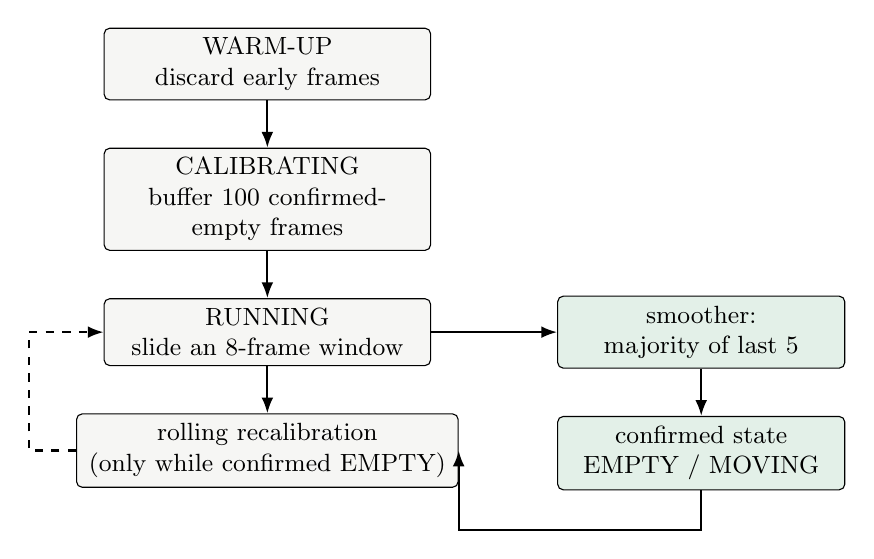
\begin{tikzpicture}[font=\small, node distance=6mm,
  b/.style={draw, rounded corners=2pt, align=center, minimum height=7mm,
            inner sep=3.5pt, fill=codebg, text width=3.9cm},
  s/.style={draw, rounded corners=2pt, align=center, minimum height=7mm,
            inner sep=3.5pt, fill=good!12, text width=3.4cm},
  a/.style={-{Latex[length=2mm]}, thick}]
\node[b] (warm) {WARM-UP\\discard early frames};
\node[b, below=of warm] (cal) {CALIBRATING\\buffer 100 confirmed-empty frames};
\node[b, below=of cal] (run) {RUNNING\\slide an 8-frame window};
\node[s, right=16mm of run] (sm) {smoother:\\majority of last 5};
\node[s, below=of sm] (conf) {confirmed state\\EMPTY / MOVING};
\node[b, below=of run, text width=4.6cm] (roll)
  {rolling recalibration\\(only while confirmed EMPTY)};
\draw[a] (warm) -- (cal);
\draw[a] (cal) -- (run);
\draw[a] (run) -- (sm);
\draw[a] (sm) -- (conf);
\draw[a] (run) -- (roll);
\draw[a] (conf.south) -- ++(0,-0.5) -| (roll.east);
\draw[a, dashed] (roll.west) -- ++(-0.6,0) |- (run.west);
\end{tikzpicture}
\caption[Real-time inference and smoothing state flow]{Live inference state
flow. The rolling calibrator observes only confirmed-empty frames, so a burst
of motion cannot contaminate the baseline. \Impl}
\label{fig:liveflow}
\end{figure}

\section{Rolling Recalibration}

The live system mirrors the per-block recalibration used during training: once
the system has been confirmed empty for a sustained period, it refreshes its
baseline rather than comparing against the startup snapshot indefinitely.

A first implementation of this drifted into predicting MOVING in an empty room,
sometimes within a single session. Two safety mechanisms were added, each
addressing a distinct failure:

\begin{enumerate}[leftmargin=1.6em, itemsep=3pt]
  \item \textbf{Blend, do not replace.} A ten-second sample is a noisy estimate
        of the true noise floor and can land quieter than typical by chance.
        Replacing the baseline outright with each such sample lets one unlucky
        quiet window ratchet sensitivity upward with nothing pulling it back. A
        weighted step toward the fresh sample ($\alpha = 0.3$) still tracks
        genuine drift over many cycles, but no single sample can dominate.
  \item \textbf{Floor against the startup baseline.} No blended standard
        deviation may fall below 60\,\% of what the original, deliberate
        ``leave the room'' calibration measured. Nothing is permitted to make
        the system \emph{more} sensitive than it ever was, only less --- so as
        to absorb a genuinely louder environment such as an air conditioner
        starting. \Impl
\end{enumerate}

\section{Two-Node OR Combination}

A single link is most sensitive to movement near the direct path between the
receiver and the access point; movement well off that axis perturbs it more
weakly. Running two physically separated receivers gives two different direct
paths, so a person in one node's weak region is frequently in the other's
strong region.

The two pipelines are entirely independent --- separate serial ports,
baselines, windows and smoothers --- and are combined with OR logic. This
requires no additional training data and no clock synchronisation between the
boards. \Impl

\begin{table}[H]
\centering
\caption{OR-combination truth table, including degraded states.}
\label{tab:orlogic}
\begin{tabular}{@{}lll l@{}}
\toprule
\textbf{Node A} & \textbf{Node B} & \textbf{Combined} & \textbf{Rationale} \\
\midrule
MOVING & EMPTY   & MOVING  & Either node suffices; this is the coverage benefit \\
EMPTY  & MOVING  & MOVING  & \\
EMPTY  & EMPTY   & EMPTY   & Only when every participating node agrees \\
MOVING & MOVING  & MOVING  & \\
EMPTY  & warming & unknown & Never infer empty from incomplete information \\
EMPTY  & OFFLINE & EMPTY   & Offline nodes are excluded entirely \\
EMPTY  & MUTED   & EMPTY   & Muted nodes are excluded entirely \\
OFFLINE& MUTED   & unknown & Nobody is voting \\
\bottomrule
\end{tabular}
\end{table}

\keyfinding{The final row is a deliberate design rule: \textbf{an empty room is
never inferred from the absence of working sensors.} This behaviour is pinned
by seventeen automated tests. \Impl}

\section{A Rejected Automatic Feature}

Because the nodes are combined with OR logic, one node producing false alarms
causes the whole system to produce them. An automatic gating mechanism was
proposed, which would use the measured noise floor to withdraw an unreliable
node's vote. It was tested before being built:

\begin{itemize}[leftmargin=1.4em, itemsep=2pt]
  \item Increasing the smoothing window from five to nine moved the false-alarm
        rate from 12.6\,\% to 12.7\,\% --- no useful effect.
  \item The noise floor correlates with false-alarm rate at only $-0.50$.
  \item Decisively: two sessions with almost identical noise floors, 0.216 and
        0.221, had false-alarm rates of \textbf{0.7\,\%} and \textbf{26.3\,\%}.
        \Repo
\end{itemize}

\noindent
The noise reading therefore cannot identify which node will misbehave, and an
automatic mechanism would have silenced sound nodes as often as faulty ones. A
\emph{manual} mute control was implemented instead. \Impl

\section{Embedded Deployment}

Training remains on the host; only inference was moved to the device. The full
200-tree forest packs to approximately 430\,kB of C, about 2.7\,\% of the
available flash, so there was no reason to prune it --- the board runs
\emph{exactly} the forest that was validated offline, which is why every
accuracy figure in this report continues to describe the hardware.

\begin{table}[H]
\centering
\caption{Verification of the embedded port.}
\label{tab:embedded}
\begin{tabularx}{\linewidth}{@{}Xr@{}}
\toprule
\textbf{Check} & \textbf{Result} \\
\midrule
Generated C simulation against the reference implementation, all windows &
\textbf{3\,302 / 3\,302} identical \\
On-device boot self-test, predictions & \textbf{12 / 12} identical \\
On-device boot self-test, features within tolerance & \textbf{266 / 266} \\
Single-precision against double-precision, all windows &
\textbf{0} prediction changes \\
Serial \code{CSI\_AMP} stream unchanged by the addition & verified by diff \\
\bottomrule
\end{tabularx}
\end{table}

\noindent
Because no host C compiler was available, the self-test embeds real recorded
frames together with the host's answers and recomputes the baseline, all 266
features and the prediction from scratch at boot. This turned out to be the
stronger choice: it exercises the actual floating-point unit and the actual
cross-compiler, which is precisely where a port of this kind fails. One
self-test vector is deliberately a window that the model classifies
\emph{incorrectly}, and the device reproduces the same incorrect answer --- the
test verifies fidelity to the reference implementation, not agreement with
ground truth. \Repo

%==============================================================================

\label{ch:method}
%==============================================================================

\section{Leave-One-Session-Out Cross-Validation}

Each of the ten recording sessions is held out in turn, a model is trained on
the remaining nine, and the held-out session is scored. Every window is
therefore classified exactly once, by a model that never saw any data from its
recording.

\begin{figure}[H]
\centering
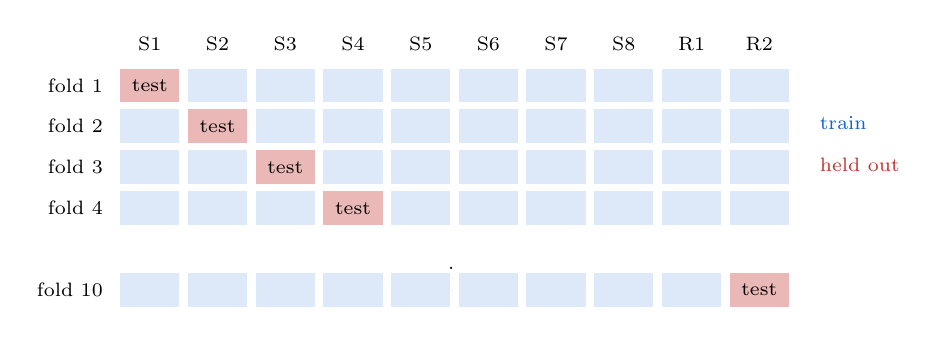
\begin{tikzpicture}[font=\scriptsize, x=0.86cm, y=0.52cm]
\foreach \r in {1,...,4} {
  \foreach \c in {1,...,10} {
    \pgfmathparse{int(\r==\c ? 1 : 0)}
    \ifnum\pgfmathresult=1
      \fill[bad!35] (\c,-\r) rectangle ++(0.9,0.86);
      \node at (\c+0.45,-\r+0.43) {test};
    \else
      \fill[accent!14] (\c,-\r) rectangle ++(0.9,0.86);
    \fi
    \draw[white, line width=0.6pt] (\c,-\r) rectangle ++(0.9,0.86);
  }
  \node[anchor=east] at (0.9,-\r+0.43) {fold \r};
}
\node at (5.9,-5.1) {$\vdots$};
\foreach \c in {1,...,10} {
  \pgfmathparse{int(\c==10 ? 1 : 0)}
  \ifnum\pgfmathresult=1
    \fill[bad!35] (\c,-6) rectangle ++(0.9,0.86);
    \node at (\c+0.45,-6+0.43) {test};
  \else
    \fill[accent!14] (\c,-6) rectangle ++(0.9,0.86);
  \fi
  \draw[white, line width=0.6pt] (\c,-6) rectangle ++(0.9,0.86);
}
\node[anchor=east] at (0.9,-6+0.43) {fold 10};
\foreach \c/\l in {1/S1,2/S2,3/S3,4/S4,5/S5,6/S6,7/S7,8/S8,9/R1,10/R2} {
  \node at (\c+0.45,0.45) {\l};
}
\node[anchor=west, accent] at (11.2,-1.5) {train};
\node[anchor=west, bad] at (11.2,-2.5) {held out};
\end{tikzpicture}
\caption[Leave-one-session-out evaluation scheme]{Leave-one-session-out
validation. S1--S8 are the room-1 sessions, R1--R2 the room-2 sessions. An
entire recording is held out at a time, never individual windows. \Impl}
\label{fig:loso}
\end{figure}

\section{Why a Random Split Would Be Misleading}

This is the single most important methodological point in the report.

Consecutive windows within one recording are extremely similar. They share the
room, the furniture arrangement, the hardware placement, the access point, the
minute of the day, the temperature, and therefore very nearly the same
multipath structure. A uniformly random train/test split places near-duplicate
windows on both sides of the partition. A sufficiently flexible model can then
achieve very high accuracy by effectively memorising the recording, and the
resulting score says almost nothing about whether the system will work
tomorrow.

\keyfinding{Holding out an entire \emph{session} converts the question from
``can the model recognise this recording?'' into ``can the model recognise
motion?'' Only the second question is worth answering.}

\section{Weighted versus Unweighted Fold Averages}

The ten folds contain different numbers of windows, from 150 to 600. Two
averages are therefore possible, and they disagree.

The \textbf{unweighted} mean of fold accuracies treats a 150-window session as
equal in importance to a 600-window one. This flatters the result whenever the
hardest session is also the largest --- which is exactly the case here, since
\code{room2\_part\_1\_data} is both the worst-performing fold and 18\,\% of all
windows.

The \textbf{weighted} mean is the true per-window out-of-fold accuracy: the
fraction of all windows in the dataset that were classified correctly by a
model that had never seen their session. This report uses the weighted figure
as the headline and reports both, so the gap remains visible. \Meas

\section{Metrics}

Accuracy is the headline because the classes are near-balanced. Precision and
recall are reported per class because the two error types have different
operational meanings: a false positive is a \emph{false alarm} (an empty room
reported as occupied), and a false negative is a \emph{missed detection}.
Matthews correlation coefficient and Cohen's kappa are reported as
chance-corrected summaries, and ROC/precision-recall curves characterise the
behaviour across decision thresholds.

\section{Cross-Room Protocol}

Separately from leave-one-session-out, a stricter test was run: a model was
trained on the eight Room 1 sessions only and scored once on an untouched
Room 2 session. This is the honest measure of transfer to a genuinely new
environment and is reported separately in Chapter~\ref{ch:results}. \Repo

%==============================================================================
\chapter{Performance Evaluation, Discussion and Future Work}
\label{ch:results}
%==============================================================================

\section{Headline Results}

\begin{table}[H]
\centering
\caption{Principal results. All figures were regenerated immediately before
writing by executing the project's own scripts.}
\label{tab:results}
\begin{tabularx}{\linewidth}{@{}Xr@{}}
\toprule
\textbf{Measurement} & \textbf{Value} \\
\midrule
Leave-one-session-out accuracy, per window (weighted) & \textbf{94.25\,\%} \\
Unweighted mean of the ten folds                      & 95.07\,\% \\
Standard deviation across folds                       & 3.86 pp \\
Best fold (\code{part\_3\_data})                      & 98.69\,\% \\
Worst fold (\code{room2\_part\_1\_data})              & \textbf{84.67\,\%} \\
\midrule
Balanced accuracy                                     & 94.25\,\% \\
Precision (MOVING)                                    & 93.60\,\% \\
Recall (MOVING)                                       & 94.96\,\% \\
F1 (MOVING)                                           & 94.28\,\% \\
Matthews correlation coefficient                      & 0.885 \\
Cohen's kappa                                         & 0.885 \\
ROC AUC                                               & 0.986 \\
Average precision                                     & 0.986 \\
Log loss                                              & 0.169 \\
\midrule
Mean \emph{training} accuracy across folds            & 100.00\,\% \\
Cross-room held-out (train Room 1, test Room 2)       & \textbf{82.50\,\%} \\
\midrule
Windows evaluated                                     & 3\,302 \\
Features per window                                   & 266 \\
Window length (live reaction time)                    & 0.75\,s \\
\bottomrule
\end{tabularx}
\end{table}

\section{Error Analysis}

\begin{table}[H]
\centering
\caption{Aggregated out-of-fold confusion matrix (3\,302 windows).}
\label{tab:confusion}
\begin{tabular}{@{}llrr@{}}
\toprule
& & \multicolumn{2}{c}{\textbf{Predicted}} \\
\cmidrule(l){3-4}
& & \textbf{EMPTY} & \textbf{MOVING} \\
\midrule
\multirow{2}{*}{\textbf{Actual}}
& \textbf{EMPTY}  & 1\,547 & 107 \\
& \textbf{MOVING} & 83     & 1\,565 \\
\bottomrule
\end{tabular}
\end{table}

\begin{table}[H]
\centering
\caption{Error rates by type.}
\label{tab:errors}
\begin{tabularx}{\linewidth}{@{}Xrr@{}}
\toprule
\textbf{Error type} & \textbf{Count} & \textbf{Rate} \\
\midrule
False alarm (empty reported as moving)   & 107 & 6.47\,\% of empty windows \\
Missed detection (moving reported as empty) & 83 & 5.04\,\% of moving windows \\
\midrule
Total errors & 190 & 5.75\,\% of all windows \\
\bottomrule
\end{tabularx}
\end{table}

\keyfinding{The two error types are close to balanced, with a mild bias toward
false alarms. For an intrusion-detection application this is the preferable
direction the system errs toward reporting occupancy rather than missing
it but a 6.47\,\% per-window false-alarm rate is far too high to act on
directly, which is why the live system requires several consecutive seconds of
agreement before raising an alert. \Meas}

\begin{figure}[H]
\centering
\projfig{0.5}{01_confusion_matrix.png}
\caption[Aggregated out-of-fold confusion matrix]{Aggregated out-of-fold
confusion matrix. \Meas}
\label{fig:cm}
\end{figure}

\begin{figure}[H]
\centering
\projfig{0.5}{02_confusion_matrix_normalized.png}
\caption[Normalised confusion matrix]{Row-normalised confusion matrix,
expressing each cell as a proportion of the true class. \Meas}
\label{fig:cmnorm}
\end{figure}

\section{Per-Session Results}

\begin{table}[H]
\centering
\caption{Leave-one-session-out results per session.}
\label{tab:perfold}
\begin{tabular}{@{}rlrrrrr@{}}
\toprule
\textbf{Fold} & \textbf{Held-out session} & \textbf{Train} & \textbf{Test} &
\textbf{Train acc.} & \textbf{Test acc.} & \textbf{Weighted F1} \\
\midrule
1  & \code{part\_1\_data}        & 3\,152 & 150 & 1.0000 & 0.9600 & 0.9599 \\
2  & \code{part\_2\_data}        & 3\,002 & 300 & 1.0000 & 0.9867 & 0.9867 \\
3  & \code{part\_3\_data}        & 2\,997 & 305 & 1.0000 & \textbf{0.9869} & 0.9869 \\
4  & \code{part\_4\_data}        & 3\,002 & 300 & 1.0000 & 0.9567 & 0.9566 \\
5  & \code{part\_5\_data}        & 3\,002 & 300 & 1.0000 & 0.9533 & 0.9532 \\
6  & \code{part\_6\_data}        & 3\,005 & 297 & 1.0000 & 0.9428 & 0.9426 \\
7  & \code{part\_7\_data}        & 3\,002 & 300 & 1.0000 & 0.9400 & 0.9398 \\
8  & \code{part\_8\_data}        & 3\,002 & 300 & 1.0000 & 0.9500 & 0.9499 \\
9  & \code{room2\_part\_1\_data} & 2\,702 & 600 & 1.0000 & \textbf{0.8467} & 0.8460 \\
10 & \code{room2\_part\_2\_data} & 2\,852 & 450 & 1.0000 & 0.9844 & 0.9844 \\
\midrule
\multicolumn{5}{r}{\textbf{Weighted mean}}   & \textbf{0.9425} & \\
\multicolumn{5}{r}{Unweighted mean}          & 0.9507 & \\
\bottomrule
\end{tabular}
\end{table}

\begin{figure}[H]
\centering
\projfig{0.9}{04_test_accuracy_by_fold.png}
\caption[Held-out accuracy by fold]{Held-out accuracy for each session. The
spread is the result, not the mean: a 94.25\,\% average contains a fold at
84.67\,\%. \Meas}
\label{fig:foldacc}
\end{figure}

\begin{figure}[H]
\centering
\projfig{0.78}{05_boxplot_fold_accuracies.png}
\caption[Distribution of fold accuracies]{Distribution of the ten fold
accuracies, showing the single low outlier. \Meas}
\label{fig:foldbox}
\end{figure}

\begin{figure}[H]
\centering
\projfig{0.9}{20_fold_performance_summary.png}
\caption[Per-fold performance summary]{Per-fold summary across several metrics.
\Meas}
\label{fig:foldsummary}
\end{figure}

\section{Threshold Behaviour}

\begin{figure}[H]
\centering
\projfig{0.7}{09_roc_curve.png}
\caption[ROC curve]{Receiver operating characteristic over the aggregated
out-of-fold predictions, with an area under the curve of 0.986. \Meas}
\label{fig:roc}
\end{figure}

\begin{figure}[H]
\centering
\projfig{0.7}{10_pr_curve.png}
\caption[Precision-recall curve]{Precision-recall curve, average precision
0.986. \Meas}
\label{fig:pr}
\end{figure}

\section{Environmental Dependence}
\label{sec:noiseresults}

The variation between folds is not random. It tracks a directly measurable
property of the recording environment: how disturbed the room is while
\emph{empty}.

\subsection*{Definition}

The metric is the mean frame-to-frame amplitude change while the room is empty,
\emph{divided by} the mean amplitude:
\begin{equation}
  N = \frac{E}{A}, \qquad
  E = \frac{1}{T-1}\sum_{t}\frac{1}{K}\sum_{k}\bigl|A_k(t+1)-A_k(t)\bigr|,
  \qquad
  A = \frac{1}{|\mathcal{K}_{\mathrm{act}}|}\!\!\sum_{k \in \mathcal{K}_{\mathrm{act}}}\!\!\bar{A}_k ,
  \label{eq:noise}
\end{equation}
where $\mathcal{K}_{\mathrm{act}}$ is the set of active (non-guard-band)
subcarriers. $N$ is dimensionless: it expresses jitter as a \emph{fraction of
received signal} rather than in raw amplitude units.

\subsection*{Why the division is necessary}

The first version of this metric used $E$ alone. That is adequate for watching
one board over time but wrong for comparing two boards, and the error was found
by measurement rather than by reasoning. Two boards were placed at the
\emph{same} location and recorded simultaneously:

\begin{table}[H]
\centering
\caption{Two receivers at the same physical location.}
\label{tab:nodeab}
\begin{tabular}{@{}lrrrr@{}}
\toprule
\textbf{Board} & \textbf{RSSI (dBm)} & \textbf{Mean amplitude} &
\textbf{Raw jitter $E$} & \textbf{Relative $N$} \\
\midrule
Node A & $-47.0$ & 32.1 & 1.63 & \textbf{0.051} \\
Node B & $-59.3$ & 16.6 & 1.17 & \textbf{0.071} \\
\bottomrule
\end{tabular}
\end{table}

\keyfinding{Node B receives 12\,dB less signal, so its amplitudes --- and hence
its raw frame-to-frame differences --- are proportionally smaller. On the raw
scale it therefore appears \emph{cleaner} than node A, while in fact it is
about \textbf{39\,\% noisier relative to what it receives}. Dividing by
amplitude makes the two comparable. This was a defect in the measurement
design, not in the system being measured. \Repo}

\subsection*{Measured values}

\begin{table}[H]
\centering
\caption{Empty-room noise floor per session, with class separation and held-out
accuracy, ordered by noise floor.}
\label{tab:noise}
\begin{tabular}{@{}lrrrl@{}}
\toprule
\textbf{Session} & \textbf{Noise floor $N$} & \textbf{Separation} &
\textbf{Accuracy} & \textbf{Grade} \\
\midrule
\code{part\_1\_data}        & 0.0249 & 4.66$\times$ & 96.00\,\% & quiet \\
\code{part\_4\_data}        & 0.0258 & 3.80$\times$ & 95.67\,\% & quiet \\
\code{part\_2\_data}        & 0.0312 & 3.13$\times$ & 98.67\,\% & quiet \\
\code{part\_3\_data}        & 0.0357 & 2.88$\times$ & 98.69\,\% & quiet \\
\code{part\_5\_data}        & 0.0445 & 5.95$\times$ & 95.33\,\% & quiet \\
\code{part\_7\_data}        & 0.0996 & 1.36$\times$ & 94.00\,\% & moderate \\
\code{room2\_part\_2\_data} & 0.1375 & 1.89$\times$ & 98.44\,\% & moderate \\
\code{part\_8\_data}        & 0.2163 & 0.99$\times$ & 95.00\,\% & loud \\
\code{part\_6\_data}        & 0.2209 & 1.02$\times$ & 94.28\,\% & loud \\
\code{room2\_part\_1\_data} & 0.2209 & 1.02$\times$ & \textbf{84.67\,\%} & loud \\
\bottomrule
\end{tabular}
\end{table}

\begin{figure}[H]
\centering
\projfig{0.95}{24_noise_floor_per_session.png}
\caption[Noise floor per session]{Measured empty-room noise floor for every
session, against the two graded thresholds. The floor varies by approximately a
factor of nine across the dataset. \Meas}
\label{fig:noisebar}
\end{figure}

\begin{figure}[H]
\centering
\projfig{0.95}{25_noise_floor_vs_accuracy.png}
\caption[Held-out accuracy against noise floor]{Held-out accuracy against
measured noise floor. The relationship is real in aggregate ($r = -0.58$) but
weak per session: the two sessions at $N \approx 0.22$ scored 94.28\,\% and
84.67\,\%. \Meas}
\label{fig:noisescatter}
\end{figure}

\keyfinding{A loud noise floor is a \textbf{risk indicator, not a forecast}.
Grouped, the effect is real --- 87.8\,\% within loud sessions against 94.1\,\%
within quiet ones --- but it does not predict the outcome of any individual
session. \Meas\ \Repo}

\subsection*{Why loud rooms are hard}

Table~\ref{tab:noise} shows the mechanism in the ``separation'' column: the
ratio of mean moving energy to mean empty energy falls from 4.66$\times$ in the
quietest session to almost exactly 1 in the loudest. When that ratio reaches 1,
the aggregate motion signal has vanished entirely and the classes can be
separated only through finer per-subcarrier structure.

\begin{figure}[H]
\centering
\projfig{1.0}{23_class_separation_quiet_vs_loud.png}
\caption[Class separation, quiet versus loud]{Distribution of per-frame motion
energy by class, for the quietest and loudest sessions. In the quiet session
the classes are clearly separated; in the loud session the two distributions
overlap almost completely, and both are bimodal. \Meas}
\label{fig:separation}
\end{figure}

\section{Learning Curve}

\begin{figure}[H]
\centering
\projfig{0.86}{14_learning_curve.png}
\caption[Learning curve]{Learning curve over training-set size. \Meas}
\label{fig:learncurve}
\end{figure}

\begin{figure}[H]
\centering
\projfig{0.86}{03_train_vs_test_by_fold.png}
\caption[Training versus test accuracy by fold]{Training against held-out
accuracy for each fold. Training accuracy is 1.0000 in every fold. \Meas}
\label{fig:traintest}
\end{figure}

\keyfinding{The forest fits its training data \textbf{perfectly} in all ten
folds, giving a train-test gap of 5.75 percentage points. This is expected for
an unpruned Random Forest and is not by itself evidence of harmful overfitting
--- bagging controls variance --- but it does mean training accuracy carries no
information here, and only the held-out figures should be quoted. \Meas}

%==============================================================================

\label{ch:discussion}
%==============================================================================

\section{Interpretation of the Headline Result}

A weighted out-of-fold accuracy of 94.25\,\% across ten sessions and two rooms
establishes that amplitude-only CSI from a single low-cost receiver carries
enough information to separate an empty room from an occupied, moving one, when
the model is calibrated against a recent empty-room baseline.

However, the mean should not be quoted alone. The distribution in
Figure~\ref{fig:foldacc} is effectively bimodal in character: seven sessions
fall between 94\,\% and 99\,\%, one falls to 84.67\,\%, and the difference
between them is not random.

\section{A New Measurement: Loud Rooms Burst}

Section~\ref{sec:noiseresults} establishes that accuracy tracks the empty-room
noise floor. A further measurement, made for this report, explains what that
noise floor actually consists of --- and it is not what the term suggests.

\begin{figure}[H]
\centering
\projfig{1.0}{27_empty_room_character.png}
\caption[Character of the empty room, quiet versus loud]{Motion energy during
the \emph{empty} blocks only, for the quietest and loudest sessions, at a
shared vertical scale. The loud session is not uniformly noisy: it alternates
between a quiet state and a disturbed one. \Meas}
\label{fig:burst}
\end{figure}

\begin{table}[H]
\centering
\caption{Character of the empty-room signal in the loud sessions.}
\label{tab:burst}
\begin{tabular}{@{}lrrrr@{}}
\toprule
\textbf{Session} & \textbf{Mean} & \textbf{Median} &
\textbf{Frames above 5} & \textbf{Median burst length} \\
\midrule
\code{part\_1\_data} (quiet)    & 0.83 & 0.79  & 0.0\,\%  & --- \\
\code{room2\_part\_1\_data}     & 5.06 & 1.20  & 41.8\,\% & 2 frames \\
\code{part\_6\_data}            & 5.87 & 1.55  & 47.8\,\% & 2 frames \\
\code{part\_8\_data}            & 5.89 & 1.33  & 49.0\,\% & 2 frames \\
\bottomrule
\end{tabular}
\end{table}

\keyfinding{In the worst session the empty room has a \textbf{median} energy of
1.20 against a \textbf{mean} of 5.06. About 42\,\% of empty frames burst to
levels indistinguishable from human movement, in short bursts with a median
length of two frames (0.2\,s). The bursts are spread evenly across all four
empty blocks (43.6\,\%, 44.2\,\%, 40.3\,\%, 39.2\,\%), so this is not one
contaminated recording but a persistent property of the environment. \Meas}

\noindent
Two consequences follow.

\textbf{The noise-floor metric averages over a bimodal signal.} Because
Equation~\ref{eq:noise} uses the mean, it describes neither the quiet state nor
the disturbed one. A median-based variant would report a very different
grading --- \code{part\_6\_data} would move from 0.221 to a value near the
quiet threshold --- and which is more useful depends on the purpose. This is
identified as a concrete improvement in Chapter~\ref{ch:improve}.

\textbf{The cause was not identified.} RSSI is essentially identical between
the quiet and bursting states ($-51.90$ against $-51.86$\,dBm in
\code{room2\_part\_1\_data}), so the total received power is stable while the
\emph{channel structure} toggles. That rules out the simplest explanation of
two different frame types being received with different signal strength, but it
does not establish what does cause it. Investigating this is proposed as future
work. \Fut

\section{Why Cross-Room Transfer Degrades}

The cross-room result --- 82.50\,\% when trained on Room 1 only and scored on an
untouched Room 2 session, against 94.25\,\% once Room 2 data are included ---
places a concrete cost on environmental change: approximately \textbf{12
percentage points until data from the new room is collected}.

The feature-importance analysis of Chapter~\ref{ch:features} identifies the
likely mechanism. The index-based features that the model relies on cluster
tightly around subcarriers 39--50, with \code{amp\_43\_std\_ratio} and
\code{amp\_44\_std\_ratio} among the six most important features overall. Those
indices are meaningful only because that is where Room 1's multipath placed a
sensitive spot; a different room places it elsewhere. The order-invariant
features were introduced precisely to counterbalance this, and their high
per-feature importance (3.24\,\% each) suggests they are doing useful work ---
but they evidently do not fully compensate.

\section{Comparison with the Literature}

The absolute accuracy figure is broadly consistent with published
single-link CSI motion detection results, which is unsurprising: binary motion
detection in a fixed environment is the easiest task in the CSI sensing
spectrum. Two aspects of this project's results are worth contrasting with the
usual presentation.

First, most reported figures in this area are within-environment, and many use
random splits. The 94.25\,\% here is a session-level out-of-fold figure and is
therefore not directly comparable with a within-session number, which would be
substantially higher.

Second, the literature consistently identifies cross-environment generalisation
as the open problem, and this project reproduces that finding quantitatively
rather than merely restating it.

\section{Threats to Validity}

\textbf{Single person.} The most serious threat. Every moving window in the
dataset is one individual's walking. The evaluation cannot separate ``detects a
person'' from ``detects this person's gait, height and movement style''.

\textbf{Two rooms.} A single cross-room data point establishes that transfer is
possible and costly, but not a trend.

\textbf{No permanently held-out set.} Every session eventually contributes to
the final model, so the reported figures are out-of-fold estimates rather than
measurements on data the model has never influenced.

\textbf{Single hardware model.} All results come from one board model and two
units of it, which differed from each other by 12\,dB in received strength ---
already a caution about hardware variation.

\textbf{Session count.} Ten sessions is a small sample for characterising a
relationship such as noise floor against accuracy; the $r = -0.58$ correlation
of Figure~\ref{fig:noisescatter} rests on ten points and should be treated as
indicative.

%==============================================================================

\label{ch:privacy}
%==============================================================================

\section{What the System Actually Records}

\begin{table}[H]
\centering
\caption{Data recorded by the system.}
\begin{tabularx}{\linewidth}{@{}lXX@{}}
\toprule
\textbf{Data} & \textbf{Where it is held} & \textbf{What it reveals} \\
\midrule
CSI amplitudes (128 values at 10\,Hz) & Session CSVs; transiently in RAM &
The radio environment. Enough to infer when a room was occupied and when
someone was moving \\
RSSI & Same & Signal strength \\
Timestamps & Same & \textbf{Exact wall-clock times} of every recorded block \\
Labels & Same & Which periods were empty or occupied \\
Wi-Fi credentials & \code{wifi\_secrets.h}, and compiled into the firmware
binary & Network access \\
\bottomrule
\end{tabularx}
\end{table}

\keyfinding{A recorded CSI dataset is \textbf{activity data about a real
room}. Combined with its timestamps, \code{all\_csi\_data.csv} shows when the
room was empty and when a person was moving in it, minute by minute. It is not
anonymous with respect to the household that produced it.}

\section{The Privacy Claim, Stated Correctly}

It is common to describe CSI sensing as privacy-preserving. That claim requires
care. The system captures no image and no audio, which removes the most obvious
class of harm and is a genuine advantage over a camera. But it does not follow
that the measurements are innocuous: the research literature has repeatedly
shown that wireless channel measurements can reveal coarse activity, gait and
even respiration.

The defensible claim is therefore narrow: \emph{this system avoids the specific
privacy problems of a camera}, and \emph{this particular implementation
extracts only a binary motion decision}. It is not a claim that CSI is
inherently private, and a richer model operating on the same recordings could
extract considerably more.

\section{Credential Handling}

\code{firmware/main/wifi\_secrets.h} contains a real SSID and password and is
listed in \code{.gitignore}; only a placeholder template is committed. Note
that credentials are also \emph{compiled into the firmware binary}, so built
images should not be distributed. \Impl

In the alerting subsystem, the mail password is read from an environment
variable and is deliberately \emph{not} accepted as a command-line argument,
because arguments are visible to every other process on the machine and are
written into shell history. An automated test asserts that no such flag exists.
\Impl

\section{Ethical Considerations for Deployment}

Deploying this system in a space used by other people raises consent questions
that are independent of the technology's capabilities. Because the sensing is
invisible --- there is no camera to see and no indicator that measurement is
occurring --- occupants cannot infer that they are being monitored. Any
deployment beyond the author's own space should involve explicit notification
of everyone who uses the room. This report makes no claim that such
notification was obtained for any environment other than the author's own.

%==============================================================================

\label{ch:limits}
%==============================================================================

\section{Scope Limitations}

\begin{table}[H]
\centering
\caption{Honest statement of what has and has not been established.}
\label{tab:limits}
\begin{tabularx}{\linewidth}{@{}lX@{}}
\toprule
\textbf{Dimension} & \textbf{Status} \\
\midrule
\textbf{People} & \textbf{One.} All training data is a single person's
movement. A second person has never been tested. This is the largest
outstanding gap and the most likely source of overestimated performance. \\
Movement styles & One --- that person's ordinary walking. \\
Rooms & Two. Cross-room transfer measured once, at 82.50\,\%. \\
Receivers & One board model, two units, differing by 12\,dB. \\
Access points & Not systematically varied. \\
Held-out data & \textbf{No permanently held-out set.} \\
Motionless occupant & \textbf{Not detectable}; classified as EMPTY. \\
Multiple occupants & Not distinguished; two read the same as one. \\
Position & Not measured. A two-zone classifier exists in the codebase but
\textbf{no zone data has ever been recorded}, so it is entirely unproven. \\
Through-wall operation & Untested and not claimed. \\
Unattended operation & Not burn-tested over long periods. \\
Safety-critical use & Explicitly unsuitable. \\
\bottomrule
\end{tabularx}
\end{table}

\section{Failure Modes}
\begin{table}[H]
\centering
\caption{Known failure modes and their handling.}
\label{tab:failures}
\renewcommand{\arraystretch}{1.25}
\begin{tabularx}{\linewidth}{|l|X|l|}
\hline
\textbf{Failure} & \textbf{Cause and handling} & \textbf{Status} \\
\hline
192 values instead of 128 &
The access point renegotiates to a 40\,MHz channel. Fixed at the source by
pinning the station to 20\,MHz; the live system also detects the mismatch and
disables prediction for that node rather than producing nonsense. &
Fixed \\
\hline
No CSI at all &
CSI exists only when packets arrive; a stale hardcoded ping target produced
silence three times. Now taken from the DHCP lease. &
Fixed \\
\hline
Baseline goes stale &
Environmental drift. Per-block recalibration offline, blended-and-floored
rolling recalibration online. &
Mitigated \\
\hline
Dead-subcarrier ratio blow-up &
Division by a zero baseline variance. Variance floor at 10\,\% of the block
median. &
Fixed \\
\hline
One node floods false alarms &
OR logic propagates it to the whole system. Manual mute; automatic gating was
tested and rejected. &
Mitigated \\
\hline
Loud environment &
The classes stop separating in aggregate energy. Measured and reported to the
operator rather than hidden. &
Reported \\
\hline
Motionless person &
Out of scope by construction; the class is never trained. &
Inherent \\
\hline
\end{tabularx}
\end{table}

\section{On the Absence of a Permanent Test Set}

Because every session is eventually folded into training, the reported figures
are out-of-fold estimates rather than measurements on data the model has never
influenced. Leave-one-session-out is a sound estimator, and
\code{evaluate\_holdout.py} provides genuine single-shot held-out figures on
demand, but a permanently reserved session --- ideally recorded in a third
room, by a second person --- would be a stronger basis for the headline claim.
\Fut

\section{On Position Estimation}

The codebase contains a two-zone classifier which runs only when motion has
already been confirmed and which leaves the binary model untouched. It is
reported here as \emph{unproven}, not as a result: no session on disk contains
a zone label. \Meas

The script deliberately refuses to report an accuracy figure if any session
contains only one zone, because a model could then achieve near-perfect scores
by learning which \emph{session} it is looking at while knowing nothing about
position. A zone model would additionally be room-specific, since it must rely
on exactly the index-based features shown in Chapter~\ref{ch:features} not to
transfer between rooms.

%==============================================================================

\label{ch:improve}
%==============================================================================

\begin{table}[H]
\centering
\caption{Proposed improvements, ranked by expected value.}
\label{tab:improve}
\renewcommand{\arraystretch}{1.25}
\begin{tabularx}{\linewidth}{|l|X|l|}
\hline
\textbf{Rank} & \textbf{Improvement} & \textbf{Cost} \\
\hline
1 &
\textbf{Collect data from a second person.} Directly attacks the largest
threat to validity. Requires only recording time. &
Low \\
\hline
2 &
\textbf{A third room}, to convert a single cross-room data point into a
trend. &
Low \\
\hline
3 &
\textbf{A permanently held-out session}, recorded in a new room by a new
person and never used for training. &
Low \\
\hline
4 &
\textbf{A median-based or bimodality-aware noise-floor metric.} The
measurement in Chapter~\ref{ch:discussion} shows the current mean-based
metric averages over a bimodal signal and describes neither state. &
Low \\
\hline
5 &
\textbf{Identify the cause of the bursting} observed in the loud sessions.
RSSI is unchanged across the two states, so the explanation is not a simple
difference in received power. &
Medium \\
\hline
6 &
\textbf{Peer-to-peer communication between boards}, so two-node OR fusion
works without a host. &
Medium \\
\hline
7 &
\textbf{Record zone data} and evaluate it against the existing decision
gate. &
Medium \\
\hline
8 &
\textbf{Long unattended operation}, to characterise drift and false-alarm
rates over days rather than minutes. &
Medium \\
\hline
\end{tabularx}
\end{table}

\noindent
All eight are \Fut. Items 1--4 are inexpensive and would materially strengthen
the claims this report is able to make.

%==============================================================================

\label{ch:future}
%==============================================================================

\section{Extending the Task}

The natural extensions in increasing order of difficulty are presence detection
(distinguishing a stationary person from an empty room, which requires
detecting respiration-scale channel variation rather than gross motion),
activity classification, and coarse zone localisation. The last of these has
scaffolding in the repository but no data. \Fut

\section{Improving Generalisation}

The measured cost of a new room is roughly 12 percentage points. Approaches
worth investigating include collecting more rooms, developing further
order-invariant representations, and domain adaptation techniques that
explicitly align feature distributions between environments. The evidence in
Chapter~\ref{ch:features} --- that the model leans on subcarriers 39--50 ---
suggests that constraining or regularising away index-specific reliance may be
productive. \Fut

\section{Deep Learning}

A convolutional or recurrent model operating directly on the windowed amplitude
matrix would remove the hand-designed feature step. This was not attempted, and
this report makes no claim about whether it would perform better. Given 3\,302
windows from ten sessions, the dataset is small for such models, and the
session-level validation used here would be essential to avoid an
over-optimistic result. \Fut

\section{Hardware Directions}

Multi-antenna receivers would expose spatial diversity and usable phase, which
is the prerequisite for genuine localisation. Deploying at 5\,GHz, or with more
than two nodes, would also be informative. \Fut

%==============================================================================

\label{ch:conclusion}
%==============================================================================

This project designed, implemented and evaluated a device-free human motion
detection system built on Wi-Fi Channel State Information and a single
low-cost ESP32-S3 microcontroller. A complete pipeline was constructed:
firmware that acquires CSI and streams per-subcarrier amplitude; a calibration
scheme that expresses every observation relative to a recent empty-room
baseline; a 266-dimensional feature representation combining per-subcarrier
statistics with deliberately order-invariant band summaries; a Random Forest
classifier selected by comparison against five alternatives; and two real-time
front ends, including one that runs the identical model on the microcontroller
itself with verified numerical parity.

Evaluated with leave-one-session-out cross-validation over ten sessions in two
rooms, the system achieves \textbf{94.25\,\%} per-window out-of-fold accuracy,
with 107 false alarms and 83 missed detections across 3\,302 windows.

The most defensible conclusion of the work, however, is methodological rather
than numerical:

\keyfinding{A single accuracy figure is the wrong way to characterise a Wi-Fi
sensing system. Performance is governed by a measurable property of the
environment --- the empty-room noise floor --- which varies by roughly a factor
of nine across this project's own recordings and corresponds to held-out
accuracy between 84.67\,\% and 98.69\,\%. A system of this kind should measure
that property and report which regime it is operating in, rather than
presenting a single number and degrading silently when conditions change.}

\noindent
This report has also documented what the system does \emph{not} do. It detects
motion, not presence: a motionless person reads as an empty room. It does not
localise, count or identify. It has been trained and tested on a single
person's movement, so the evaluation cannot distinguish detecting \emph{a}
person from detecting \emph{this} person. And its cross-room transfer, measured
once, costs approximately twelve percentage points.

The single most valuable next step is inexpensive and unambiguous: record
movement data from additional people. Until that is done, the central claim of
any system of this kind remains untested.

%==============================================================================
\begin{thebibliography}{9}
\addcontentsline{toc}{chapter}{References}
%==============================================================================

\bibitem{espidf}
Espressif Systems,
\emph{ESP-IDF Programming Guide}, version 6.0.
\url{https://docs.espressif.com/projects/esp-idf/en/stable/esp32s3/}

\bibitem{sklearn}
scikit-learn developers,
\emph{scikit-learn: Machine Learning in Python}.
\url{https://scikit-learn.org/}

\bibitem{ieee80211}
IEEE Standard for Information Technology,
\emph{IEEE 802.11: Wireless LAN Medium Access Control (MAC) and Physical Layer
(PHY) Specifications}.

\bibitem{yadav2022csitime}
S. K. Yadav, S. Sai, A. Gundewar, H. Rathore, K. Tiwari,
H. M. Pandey, and M. Mathur,
\emph{CSITime: Privacy-preserving human activity recognition using WiFi
channel state information},
Neural Networks, vol. 146, pp. 11--21, 2022.
doi: 10.1016/j.neunet.2021.11.011.

\bibitem{damodaran2022wifi}
N. Damodaran \emph{et al.},
\emph{Human Activity Recognition based on Wi-Fi CSI Data -- A Deep Neural
Network Approach},
Procedia Computer Science, vol. 198, pp. 59--66, 2022.
doi: 10.1016/j.procs.2021.12.211.
\bibitem{repo}

Project source code, datasets and full development history.
\url{https://github.com/IALR/csi-motion-detection}

\bibitem{repo}
Reference Repository and Development Basis.
\url{https://github.com/ruvnet/RuView}

\end{thebibliography}

%==============================================================================
\appendix
\chapter{Reproducing the Results}
\label{app:repro}
%==============================================================================

All figures and tables in this report are regenerated by the following
commands, executed from the repository root.

\begin{lstlisting}[language=bash, caption={Reproduction commands.}]
# --- environment -----------------------------------------------------------
python -m venv .venv
python -m pip install -r requirements.txt

# --- the deployed model and every headline number --------------------------
python train_model.py

# --- single-shot held-out evaluation on a named session ---------------------
python evaluate_holdout.py --test room2_part_1_data

# --- comparison of six model families under identical validation -----------
python compare_models.py

# --- the ~20 standard classifier diagnostics (figures 01-20) ---------------
python full_model_report.py --model csi_model.joblib \
    --sessions part_1_data part_2_data part_3_data part_4_data part_5_data \
               part_6_data part_7_data part_8_data \
               room2_part_1_data room2_part_2_data

# --- the project-specific figures (21-27) and the PDF figure books ---------
python make_report_figures.py

# --- the automated test suite (72 tests, no hardware required) -------------
python -m pytest tests/
\end{lstlisting}

\begin{lstlisting}[language=bash, caption={Firmware build and flash commands,
ESP-IDF v6.0.2 under Windows PowerShell.}, label={lst:idf}]
# --- open the IDF environment (needed in EVERY new PowerShell window) ------
& $env:IDF_PATH\export.ps1
idf.py --version                     # must print v6.0.2

# --- if PowerShell refuses to run the script ------------------------------
Set-ExecutionPolicy -Scope CurrentUser RemoteSigned

# --- all idf.py commands run from firmware/, not the repository root ------
cd firmware

# --- one-time setup per clone ---------------------------------------------
Copy-Item main\wifi_secrets.h.example main\wifi_secrets.h
notepad main\wifi_secrets.h          # add real SSID and password (gitignored)
idf.py set-target esp32s3            # regenerates sdkconfig from the defaults

# --- the everyday loop ----------------------------------------------------
idf.py build                         # compile and link -> build/csi_node.bin
idf.py -p COM9 flash                 # write bootloader, table and app
idf.py -p COM9 monitor               # serial console at 115200; exit Ctrl-]
idf.py -p COM9 flash monitor         # the one you actually type

# --- find the serial port -------------------------------------------------
[System.IO.Ports.SerialPort]::GetPortNames()
Get-CimInstance Win32_PnPEntity |
    Where-Object { $_.Name -match 'COM\d+' } | Select-Object Name

# --- cleaning, and confirming the four critical settings survived ---------
idf.py fullclean                     # then set-target again
Select-String -Path sdkconfig -Pattern "FLASHSIZE|PARTITION_TABLE|WS_SUPPORT"

# --- standard ESP-IDF, useful here but not documented by this project -----
idf.py menuconfig                    # inspect only: sdkconfig is generated
idf.py size                          # app is 1461504 B in a 4 MB partition
idf.py size-components               # where that size goes
idf.py partition-table               # confirm factory really is 4 MB
idf.py -p COM9 -b 460800 flash       # faster flashing baud (not monitor baud)
idf.py -p COM9 erase-flash           # destructive: wipes NVS and PHY data too
\end{lstlisting}

\noindent
\textbf{Note.} \code{train\_model.py} overwrites \code{csi\_model.joblib} by
default; use \code{--model-out} to write elsewhere when experimenting.


\begin{lstlisting}[language=bash, caption={Running the live detector: flashing
both nodes, single- and two-node operation, and alert delivery. Python commands
run from the repository root, \texttt{idf.py} from \texttt{firmware/}.},
label={lst:live}]
# --- 1. flash both boards: identical firmware, one COM port each ----------
cd firmware
idf.py -p COM9 flash                 # node A
idf.py -p COM6 flash                 # node B
cd ..

# --- 2. confirm both nodes stream before involving the model -------------
python diagnose_nodes.py -p COM9 --port-b COM6
python diagnose_nodes.py -p COM9 --port-b COM6 --seconds 60

# --- 3. single node ------------------------------------------------------
python csi_live_server.py -p COM9 -b 115200

# --- 4. two nodes, OR-combined (-b 115200 is the default, so optional) ---
python csi_live_server.py -p COM9 --port-b COM6 -b 115200

# --- 5. then open csi_dashboard.html by double-clicking it ---------------
#     no local HTTP server is needed; from file:// it connects to
#     ws://localhost:8765 on its own

# --- 6. phone push via ntfy.sh (no account; the topic IS the secret) -----
$topic = "https://ntfy.sh/csi-pick-a-long-random-topic"
python csi_live_server.py -p COM9 -b 115200 --alert-webhook $topic
python csi_live_server.py -p COM9 --port-b COM6 --alert-webhook $topic

# --- 7. check delivery without standing in a room waving ----------------
python csi_live_server.py --test-alert --alert-webhook $topic

# --- 8. email: the password comes from the environment, never a flag ----
$env:CSI_SMTP_PASS = "your_16_char_app_password"
python csi_live_server.py -p COM9 --alert-email you@example.com

# --- 9. tune the sustained hold and the cooldown (defaults 5 s, 60 s) ---
python csi_live_server.py -p COM9 --alert-seconds 5 --alert-cooldown 60
\end{lstlisting}
%==============================================================================
\chapter{Principal Source Files}
\label{app:files}
%==============================================================================

\begin{table}[H]
\centering
\caption{Principal components of the implementation.}
\begin{tabularx}{\linewidth}{@{}lX@{}}
\toprule
\textbf{File} & \textbf{Responsibility} \\
\midrule
\code{csi\_common.py} & \textbf{Single source of truth} for parsing, feature
extraction, calibration and smoothing. Imported by the training path and both
live paths so that offline and online behaviour cannot diverge. \\
\code{csi\_label\_collector.py} & Auto-cycling data collection protocol. \\
\code{train\_model.py} & Dataset construction, leave-one-session-out validation
and model persistence. \\
\code{evaluate\_holdout.py} & True single-shot held-out evaluation. \\
\code{compare\_models.py} & Six model families under identical validation. \\
\code{full\_model\_report.py} & The 20 standard diagnostic figures and metrics. \\
\code{make\_report\_figures.py} & The project-specific figures used in this report. \\
\code{csi\_live\_server.py} & Live inference, one or two nodes, OR fusion,
degraded-state handling and alerting. \\
\code{csi\_live\_predict.py} & Desktop live inference front end. \\
\code{csi\_dashboard.html} & Self-contained browser interface; also embedded
into the firmware and served by the board. \\
\code{diagnose\_nodes.py} & Distinguishes a noisy environment from a poorly
receiving board. \\
\code{export\_model\_c.py} & Exports the forest to C with verification against
the reference implementation. \\
\code{firmware/main/csi\_node.c} & CSI capture, ping trigger, serial output. \\
\code{firmware/main/csi\_features.c} & The 266 features reimplemented in C. \\
\code{tests/test\_pipeline.py} & The 72-test suite. \\
\code{docs/PROJECT\_HISTORY.md} & Full chronological development record. \\
\bottomrule
\end{tabularx}
\end{table}

%==============================================================================
\chapter{Testing}
\label{app:tests}
%==============================================================================

The project includes \textbf{72 automated tests}, none of which requires
hardware. Their focus differs from the usual emphasis in a machine-learning
project:

\keyfinding{The tests principally pin \emph{live-system failure modes} rather
than model accuracy --- malformed serial lines, a node going offline, the
access point changing channel width mid-run. Every defect this project
encountered twice was a failure-mode defect, not a mathematical one. \Impl}

\begin{table}[H]
\centering
\caption{Coverage of the automated test suite.}
\begin{tabularx}{\linewidth}{@{}lX@{}}
\toprule
\textbf{Area} & \textbf{Examples} \\
\midrule
Parsing & Valid lines, leading noise, malformed input, and verification that
the declared value count matches the number of amplitudes actually received \\
Node fusion & Seventeen truth-table cases, including that an entirely muted or
offline system reports \emph{unknown} and never EMPTY \\
Calibration & The dead-subcarrier ratio blow-up is prevented; the rolling
calibrator ignores moving frames; the floor prevents a sensitivity ratchet \\
Noise floor & The ten real sessions are graded correctly; the metric is
scale-free across receivers of differing sensitivity \\
Alerting & The hold is respected; brief bursts are ignored; the cooldown
behaves; alerts never fire on an unknown state \\
Security & The mail password must come from the environment; no password
command-line flag may exist \\
Configuration drift & Analysis scripts must not hardcode session lists; the
default window must match the deployed model \\
\bottomrule
\end{tabularx}
\end{table}

\end{document}
